% !TeX document-id = {8ff48607-dcb4-4d5c-89b6-63c6d50da873}
% !BIB TS-program = biber
\documentclass[12 pt,a4paper,oneside]{book}
\usepackage[T1]{fontenc}
\usepackage[top=1in,bottom=0.7in,left=1in,right=1in]{geometry}

\usepackage[
backend=biber,
style=alphabetic,
sorting=ynt
]{biblatex}
\addbibresource{references.bib}

\usepackage{amsfonts,amsmath,amsthm,amssymb}
\theoremstyle{plain}

\usepackage{float,mathtools,dirtytalk,ulem,csquotes,cancel,hyperref}

% plotting things
\usepackage{graphicx,tikz,tikz-3dplot}
\graphicspath{{images/}}
\usepackage{pst-solides3d,tikz-cd}
\usetikzlibrary{positioning, decorations.markings, calc,intersections,fadings, shadows.blur,patterns,arrows}
\usepackage{forest,svg}
\usepackage{pgfplots}
\usepgfplotslibrary{patchplots}
\pgfplotsset{compat=1.15}


\usepackage{xcolor}
\definecolor{fg}{RGB}{30,30,30}
\newcommand{\semitransp}[2][80]{\textcolor{fg!#1}{#2}}

% from amsthm package
\newtheorem{theorem}{Theorem}[section]
\theoremstyle{definition}
\newtheorem{conjecture}{Conjecture}[section]
\newtheorem{definition}{Definition}[section] % make dependence on theorem numbers
\newtheorem{example}{Example}[section]
\newtheorem{problem}{Problem}[section]
\newtheorem{extra}{Extra}[section]
\newtheorem{proposition}{Proposition}[section]
\numberwithin{equation}{section} % Number equations within sections

% Add triangle at the end of the example
\AtBeginEnvironment{example}{%
  \pushQED{\qed}\renewcommand{\qedsymbol}{$\triangle$}%
}
\AtEndEnvironment{example}{\popQED\endexample}

\usepackage[toc,page]{appendix}
\usepackage{relsize}

% Set pdfborder option to remove red box
\hypersetup{colorlinks=true,linkcolor=black}


% add style for chapter
\usepackage{fancyhdr,lastpage,lipsum,caption,subcaption,enumitem,setspace,forest}
% box
\usepackage{environ}
\usepackage{xcolor}
\usepackage[tikz]{bclogo}
\usepackage{tikz}
\usetikzlibrary{calc}
\NewEnviron{myremark}[1]
  {\par\medskip\noindent
  \begin{tikzpicture}
    \node[inner sep=0pt] (box) {\parbox[t]{.99\textwidth}{%
      \begin{minipage}{.3\textwidth}
      \centering\tikz[scale=5]\node[scale=3,rotate=30]{\bclampe};
      \end{minipage}%
      \begin{minipage}{.65\textwidth}
      \textbf{#1}\par\smallskip
      \BODY
      \end{minipage}\hfill}%
    };
    \draw[red!75!black,line width=3pt] 
      ( $ (box.north east) + (-5pt,3pt) $ ) -- ( $ (box.north east) + (0,3pt) $ ) -- ( $ (box.south east) + (0,-3pt) $ ) -- + (-5pt,0);
    \draw[red!75!black,line width=3pt] 
      ( $ (box.north west) + (5pt,3pt) $ ) -- ( $ (box.north west) + (0,3pt) $ ) -- ( $ (box.south west) + (0,-3pt) $ ) -- + (5pt,0);
  \end{tikzpicture}\par\medskip%
}

\usepackage{lmodern,wasysym}
\usepackage[most]{tcolorbox}
\usepackage{nicematrix}

\usepackage{bm}
\pagestyle{fancy}
\lhead{Section \thesection}
\rhead{Page \thepage}
\cfoot{}
%\usepackage[Glenn]{fncychap}






\usepackage{physics}
\usepackage[outline]{contour} % glow around text
\usetikzlibrary{angles,quotes} % for pic
\tikzset{>=latex} % for LaTeX arrow head
\usepackage{xcolor}
\colorlet{veccol}{green!70!black}
\colorlet{vcol}{green!70!black}
\colorlet{xcol}{blue!85!black}
\colorlet{projcol}{xcol!60}
\colorlet{unitcol}{xcol!60!black!85}
\colorlet{myblue}{blue!70!black}
\colorlet{myred}{red!90!black}
\colorlet{mypurple}{blue!50!red!80!black!80}
\tikzstyle{vector}=[->,very thick,xcol]

%% start writing the content %%

\begin{document}
\begin{titlepage}
	\begin{center}
		\vspace*{1cm}
		\Huge
		\textbf{MAT216: Linear Algebra \& Fourier Analysis}
	\end{center}
	\onehalfspacing
	\begin{center}
		\vfill
		{ \Large Lecture Notes}
		\vfill
		{ \Large
			Course Instructor \\
			\textbf{Emon Hossain} \\
			% April, 2024 \\
		}
		\vfill
		% { \Large
			% 	Under the Direct Supervision of \\[0.2 cm]
		\vfill
		\includegraphics[scale=0.5]{brac-university-logo.png}
		\vfill
		{ \Large
			\textbf{Mathematics and Natural Sciences}\\
			BRAC University \\
			Dhaka, Bangladesh \\
		}
		\vfill
		\vspace{30pt}
	\end{center}
\end{titlepage}
\clearpage
\pagenumbering{roman}
\chapter*{Acknowledgement}
This series of lecture notes has been prepared to aid students who took the BRAC University
course Linear Algebra \& Fourier Analysis (MAT216) in the Summer 2024 semester. 
%I would like to thank my students Arafat and Chowdhury Zawad Al Munawar for their considerable help with a preliminary draft in \LaTeX.
The main goal of this typeset is to have an organized digital version of the notes, which is easier to share and handle. Of course, any mistakes in this text are entirely mine. I only hope to provide an easy-to-read introduction. Proofs will be omitted if the required mathematics are beyond the scope of this course. Many times only an example or an intuitive outline will be given. I am certain that some of my reasoning won't hold in a thorough mathematical review, but at least you should get an impression. If you see any mistakes or typos, please send me an email at \href{mailto:emon.hossain@bracu.ac.bd}{emon.hossain@bracu.ac.bd} with the subject: \textbf{Correction on page \# [MAT216 Lecture note]}. 
\pagebreak
\tableofcontents
\pagebreak
\hypersetup{urlcolor=green,citecolor=red,linkcolor=blue}
\pagenumbering{arabic}
\setcounter{page}{1}

\chapter{Lecture 1}
\section{Motivation}
System of equations is the most fascinating topic in Linear Algebra. Because we can see it through both vector space and Linear Transformation perspective respectively. For example, take a system of linear equations,
\begin{align}
\begin{split}
    x-y&=1\\
    2x+y&=6
\end{split}
\end{align}
If you write the system as a linear combination of vectors (as we are considering our coefficient of a specific variable e.g., $\begin{pmatrix}
    1\\2
\end{pmatrix}$ for $x$ to a column vector which live in $\mathbb R^2$) then we can rewrite it as,
\begin{align*}
    \begin{pmatrix}
        1\\2
    \end{pmatrix}x+\begin{pmatrix}
        -1\\1
    \end{pmatrix}y=\begin{pmatrix}
        1\\6
    \end{pmatrix}
\end{align*}
\textbf{Interpretation of the solution:} Here, we want to find such scalars $x,y$ for which our vectors $\begin{pmatrix}
    1\\2
\end{pmatrix}$ and $\begin{pmatrix}
    -1\\1
\end{pmatrix}$ can reach the vector $\begin{pmatrix}
    1\\6
\end{pmatrix}$ by \textbf{vector addition}.
\\~\\
Likewise, we can rewrite the system as,
\begin{align*}
    \begin{pmatrix}
        1 & -1\\
        2 & 1
    \end{pmatrix}\begin{pmatrix}
        x\\y
    \end{pmatrix}=\begin{pmatrix}
        1\\6
    \end{pmatrix}
\end{align*}
Here, we are considering the linear transformation (don't worry we will discuss it in our upcoming lectures, or if you want to understand it right now have a look at the course \href{https://www.youtube.com/watch?v=fNk_zzaMoSs&list=PLZHQObOWTQDPD3MizzM2xVFitgF8hE_ab}{Essence of linear algebra}, YouTube playlist from 3b1b channel) and want to find such vectors which are mapped to the specific vector $\begin{pmatrix}
    1\\6
\end{pmatrix}$ after the transformation applied.\\
\textbf{Interpretation of the solution:} So, basically we want all those vectors $\begin{pmatrix}
    x\\y
\end{pmatrix}$ which are mapped to $\begin{pmatrix}
    1\\6
\end{pmatrix}$.
\clearpage
\begin{center}
	\begin{forest}
		for tree={%
			align=center, %% ADDED
			edge path={\noexpand\path[\forestoption{edge}] (\forestOve{\forestove{@parent}}{name}.parent anchor) -- +(0,-12pt)-| (\forestove{name}.child anchor)\forestoption{edge label};}
		}
		[
		System of linear Equations,
		[Algebraic form]
		[Vector form]
		[Transformation form]
        [$\cdots$]
		]
	\end{forest}
\end{center}



\begin{figure}[H]
\centering
\includegraphics[scale=0.3]{images/madness.jpeg}
\end{figure}
Welcome to Linear Algebra, where the notation is made up and you might gain your third eye.
\begin{displayquote}
\say{Life isn't linear, but written words are. Like our system of linear equations.}
\end{displayquote}

\section{System of Linear Equations} 
Let's Consider,
\begin{align*}
    3x&=6\\
    2y&=4
\end{align*}
We can easily find the solution of this two-dimensional linear equation or a system of equations where($x=2$ and $y=2$). Because the equations of this system (lines) are orthogonal or in other words, they are perpendicular to each other.

% you can use this template to add image
\begin{figure}[H]
\centering
\includegraphics[scale=0.5]{L1 example 1.png}
\end{figure}
~\\
\textbf{Remark:} In this course, our main focus will be to convert any system of linear equations into an orthogonal set of linear equations (which might not look the same but share the same solution). And how will we do this? Gaussian Elimination! Gaussian Elimination!! Gaussian Elimination!!! 

\subsection{System of equation: Two variables}
For two-dimensional linear equations, there are two different possible types. Either it is: \emph{Consistent} or \emph{Inconsistent}. Consistent means that, the system may have unique or multiple solutions whereas inconsistent means there is no possible solution for the system.

\begin{figure}[H]
\centering
\includegraphics[scale=0.9]{L1 lines.png}
\end{figure}

 If the slopes of the lines are the same then they may be parallel or they may be the same exact line. In this case, one line may be scaled or extended by a scalar multiplication. Again, if they are parallel, then there will be no solutions and again, if they are exact same line then, there will be infinitely many solutions. On the other hand, one unique solution is possible if they coincide at one point.

\subsection{System of Equation: Three variables}
A three-dimensional linear system has also three possible types of solutions.\\
 \textbf{Fact:}\\
 Every system of linear equations has zero, one, or infinitely many solutions. There are
no other possibilities.\\
But for three-dimensional cases, many possible cases will result which gives the above solution case.

\begin{figure}[H]
\centering
\includegraphics[scale=0.7]{L1 planes.png}
\end{figure}

Like for a three-variable system:
$$
\begin{cases}
    a_1x+b_1y+c_1z&=d_1\\
    a_2x+b_2y+c_2z&=d_2\\
    a_3x+b_3y+c_3z&=d_3
\end{cases}
$$
We can rewrite it in the vector form:
$$
\underbrace{\begin{pmatrix}
    a_1\\a_2\\a_3
\end{pmatrix}}_{\in\mathbb R_3}x+
\underbrace{\begin{pmatrix}
    b_1\\b_2\\b_3
\end{pmatrix}}_{\in\mathbb R_3}y+
\underbrace{\begin{pmatrix}
    c_1\\c_2\\c_3
\end{pmatrix}}_{\in\mathbb R_3}z=
\underbrace{\begin{pmatrix}
    d_1\\d_2\\d_3
\end{pmatrix}}_{\in\mathbb R_3}
$$
So, our solution $\begin{pmatrix}
    x\\y\\z
\end{pmatrix}$ actually tell us how much we should scale our column vectors $\begin{pmatrix}
    a_1\\a_2\\a_3
\end{pmatrix},\begin{pmatrix}
    b_1\\b_2\\b_3
\end{pmatrix}$ and $\begin{pmatrix}
    c_1\\c_2\\c_3
\end{pmatrix}$ respectively in order to reach the right hand side vector $\begin{pmatrix}
    d_1\\d_2\\d_3
\end{pmatrix}$.
\\~\\
Two questions that we will revisit many times throughout our course:
\begin{enumerate}
    \item Does a given linear system have a solution? In other words, is it consistent?
    \item If it is consistent, is the solution unique?
\end{enumerate}
Let's sum up everything in a diagram:


\begin{center}
\begin{forest}
for tree={
  align=center,
  grow'=south,
  parent anchor=south,
  child anchor=north,
  l=2cm,
  s sep=10pt,
  edge={->}
}
[
\shortstack{Linear system},
  [\shortstack{Consistent},
    [\shortstack{Unique solution\\(number of unknowns\\=\\number of pivots)}]
    [\shortstack{Many solutions\\(number of unknowns\\>\\number of pivots)}]
  ]
  [\shortstack{Inconsistent},
    [\shortstack{No solution\\(zero=non-zero)}]
  ]
]
\end{forest}
\end{center}


\section{Too early for Gaussian Elimination?}
Gaussian elimination, also known as row reduction, is an algorithm for solving systems of linear equations. It consists of a sequence of row-wise operations performed on the corresponding matrix of coefficients. Rules of Gaussian Elimination:

\begin{itemize}
    \item  Multiplying by a constant.
    \item Adding a row by row
    \item Row swap
\end{itemize}

The following example is a preview of how we can say so many things just by looking at the columns. 
\begin{tcolorbox}[colback=red!5!white,colframe=red!75!black]
  \textbf{Question $1$}: Solve the following system,
  $$
  \begin{cases}
    x+4z+7t&=8\\
    y+5z+11t&=11
\end{cases}
  $$
\end{tcolorbox}
 We can write the linear system,
% use $$ code $$ to make render math mode
$$
\begin{cases}
    x+4z+7t&=8\\
    y+5z+11t&=11
\end{cases}\implies
\underbrace{\begin{pmatrix}
 1 & 0&4&7\\
 0&1&5&11\\
 \end{pmatrix}}_{\text{coefficient matrix}}\begin{pmatrix}
     x\\
     y\\
     z\\
     t\\
 \end{pmatrix} = \begin{pmatrix}
     8\\
     11\\
 \end{pmatrix}
$$ 
Now, if we consider $z=0 ,t =0$, then our system will be reduced and we will get,
$$
\begin{pmatrix}
 1 & 0\\
 0&1\\
 \end{pmatrix}\begin{pmatrix}
     x\\
     y\\
     
 \end{pmatrix} = \begin{pmatrix}
    8\\
     11\\
 \end{pmatrix}
 $$
then, we can find the solution easily, $x=8$, $y=11$.\\
But wait, the story isn't over yet. This solution isn't the sole one for this system; many possible solutions exist. Can you contemplate the underlying reason? 

\begin{myremark}{Hints:}
If you see the system through the column perspective then we have four vectors $\begin{pmatrix}
    1\\0
\end{pmatrix},\begin{pmatrix}
    0\\1
\end{pmatrix},\begin{pmatrix}
    4\\5
\end{pmatrix},\begin{pmatrix}
    7\\11
\end{pmatrix}$ in $\mathbb R^2$. And we want to reach $\begin{pmatrix}
    8\\11
\end{pmatrix}$ using those vectors. 
\end{myremark}
According to the General Formula which we didn't discuss in full detail,
$$
\text{Solution}=\begin{pmatrix}
    8\\
    11\\
    0\\
    0\\
    
\end{pmatrix} + \alpha \begin{pmatrix}
    4\\
    5\\
    -1\\
    0\\
    
\end{pmatrix} + \beta \begin{pmatrix}
    7\\
    11\\
    0\\
    -1\\
\end{pmatrix}
$$
Here we can see that the multiplication of the first column by $4$, the second one by $5$ and the third column by $-1$ give us zero vector.
$$
4\begin{pmatrix}
 1\\0   
\end{pmatrix}+5\begin{pmatrix}
    0\\1
\end{pmatrix}-\begin{pmatrix}
    4\\5
\end{pmatrix}+0\begin{pmatrix}
    7\\11
\end{pmatrix}=\begin{pmatrix}
    0\\0
\end{pmatrix}
$$
That means this configuration $4,5,-1,0$ (linear combination) of column vectors will give us $\begin{pmatrix}
    0\\0
\end{pmatrix}$. But how do we represent this linear combination? Look carefully what our solution $\begin{pmatrix}
    x\\y\\z\\t
\end{pmatrix}$ does to the column vectors.
\begin{myremark}{Hints:}
$$
\begin{pmatrix}
 1 & 0&4&7\\
 0&1&5&11\\
 \end{pmatrix}\begin{pmatrix}
     x\\y\\z\\t
 \end{pmatrix}=\begin{pmatrix}
     1\\0
 \end{pmatrix}x+\begin{pmatrix}
     0\\1
 \end{pmatrix}y+\begin{pmatrix}
     4\\5
 \end{pmatrix}z+\begin{pmatrix}
     7\\11
 \end{pmatrix}t
 $$
\end{myremark}
~\\
And adding this to our particular solution $\begin{pmatrix}
    8\\11\\0\\0
\end{pmatrix}$ won't change the solution at all. Similarly for $\begin{pmatrix}
    7\\11\\0\\-1
\end{pmatrix}$. But can you see what's going on with our solution set? 
\begin{tcolorbox}[colback=red!5!white,colframe=red!75!black]
  \textbf{Question $2$}: Solve the following system,
$$
\begin{pmatrix}
    1&2&3\\
    4&5&6\\
    7&8&9\\
\end{pmatrix}\begin{pmatrix}
    x\\
    y\\
    z\\
\end{pmatrix}=\begin{pmatrix}
    20\\50\\80
\end{pmatrix}
$$
\end{tcolorbox}
~\\
We have given that:
$$
\begin{pmatrix}
    1&2&3\\
    4&5&6\\
    7&8&9\\
\end{pmatrix}\begin{pmatrix}
    x\\
    y\\
    z\\
\end{pmatrix}=\begin{pmatrix}
    20\\50\\80
\end{pmatrix}
$$
Now, if we multiply column two by $10$ we can get a particular solution,
$\begin{pmatrix}
    x\\y\\z
\end{pmatrix}=\begin{pmatrix}
    0\\10\\0\\
\end{pmatrix}$. Because this solution gives us,
$$
\begin{pmatrix}
    1\\4\\7
\end{pmatrix}\cdot0+\begin{pmatrix}
    2\\5\\8
\end{pmatrix}\cdot10+\begin{pmatrix}
    3\\6\\9
\end{pmatrix}\cdot0=\begin{pmatrix}
    20\\50\\80
\end{pmatrix}
$$
So, $x=0, y=10, z = 0$. which is our particular solution. By the way, What if we apply Gaussian Elimination here?

$$
\left(\begin{array}{ccc|c}
     1&2&3&20\\
     4&5&6&50\\
     7&8&9&80
\end{array}\right)\stackrel{R_2'=R_2-4R_1}{\sim}
\left(\begin{array}{ccc|c}
     1&2&3&20\\
     0&-3&-6&-30\\
     0&-6&-12&-60
\end{array}\right)\stackrel{R_3'=R_3-2R_2}{\sim}
\left(\begin{array}{ccc|c}
     1&2&3&20\\
     0&-3&-6&-30\\
     0&0&0&0
\end{array}\right)
$$
If we write the general solution, we will get something like the below: 
$$
\begin{pmatrix}
    x\\y\\z
\end{pmatrix}=\begin{pmatrix}
    z\\10-2z\\z
\end{pmatrix}\implies\begin{pmatrix}
    x\\y\\z
\end{pmatrix}=
\begin{pmatrix}
    0\\10\\0
\end{pmatrix}+\begin{pmatrix}
    1\\-2\\1
\end{pmatrix}z
$$
Ah, we get more solutions, and to get more things we have to do something extra \smiley. 


\clearpage
\chapter{Lecture 2}
\section{Why does Gaussian Elimination work? No geometry, Uhem!}
There are three fundamental operations we perform on a linear system. 
\begin{itemize}
    \item Multiplying a row by a scalar. 
    \item Interchanging two rows. 
    \item Adding a scalar multiple of a row to another row. 
\end{itemize}
These are called \textbf{Elementary row operations}. The thing to notice is that after performing any of these three operations the resultant system consists of equations that are linear combinations of the original one.\\~\\ 
For example, say we have a system, 
$$
\begin{array}{c}
a_1x+b_1y+c_1z=d_1 \\ 
a_2x+b_2y+c_2z=d_2 \\ 
a_3x+b_3y+c_3z=d_3
\end{array}
$$
Say we multiply the first row by $q$ and add it to the second. The resultant system is, 
$$
\begin{array}{c}
a_1x+b_1y+c_1z=d_1 \\ 
q(a_1x+b_1y+c_1z) + a_2x+b_2y+c_2z=q \cdot d_1 + d_2 \\ 
a_3x+b_3y+c_3z=d_3
\end{array}
$$
Now say $(x, y, z)^T$ was a solution to the original system. Then, it is also a solution to the second one. Let us try to convince ourselves of this. The first and last rows are not a problem. The second equation of the resultant system is also satisfied because $a_2x+b_2y+c_2z= d_2$ and $(a_1x+b_1y+c_1z) = d_1 \implies q (a_1x+b_1y+c_1z) = q \times d_1 $. 
\\~\\
The other two linear operations are also similarly disposed of. 
\\~\\
Now look at what we have proven. We have proven that \textit{"any solution to the original system is a solution to the system resulting from one of the three linear operations"}. 
\\~\\
But we require a little more. We want the solutions of the new system to be exactly those of the first one. This is established by the fact that every linear operation mentioned has a corresponding inverse operation *which is also one of the three linear operations*. For example, the inverse operation of the one we performed above is multiplying the first row of the second system by $-q$ and adding to the second row. Now think of the original system as resulting from the second one through the performance of a linear operation. Hence from what we proved above any solution to the second system is also a solution to the first. 

So any solution to the original system is a solution to the resultant system and any solution to the resultant system is a solution to the original one. Hence the solutions to the first system are exactly those to the second. This is exactly what we require. There is a nice explanation of all this in the first twenty or so pages in \href{http://www.cin.ufpe.br/~jrsl/Books/Linear%20Algebra%20-%20Kenneth%20Hoffman%20&%20Ray%20Kunze%20.pdf}{"Linear Algebra by Hoffman, Kunze"}. 
\section{Gaussian Elimination in Action}
 If the slopes of a linear system equation are different, then the intersection point is unique.
Consider,
\begin{align*}
    x-y&=1\\
    2x+y&=6
\end{align*}

\begin{figure}[H]
\centering
\includegraphics[scale=0.3]{images/L2 S1.jpeg}
\end{figure}
~\\
 To solve a linear equation both two or three-dimensional, we try to make the equation lines orthogonal.\\
 For the above system\\~\\
\textbf{Step $1$:} by doing, $ R_2'= R_2-2R_1$\\
 $$
 \begin{pmatrix}
 x &-y\\
 0 & 3y \\
 \end{pmatrix}=\begin{pmatrix}
     1\\
     4\\
 \end{pmatrix}
$$
\textbf{Step:} $2$ by doing $R_1'=R_1+\frac{1}{3}R_2$,
$$
\begin{pmatrix}
 x &0\\
 0 & 3y \\
 \end{pmatrix}=\begin{pmatrix}
     \frac{7}{3}\\
     4\\
 \end{pmatrix}
$$
The corresponding linear system becomes:
$$
\begin{cases}
    x&=\frac73\\
    3y&=4
\end{cases}
$$
\begin{figure}[H]
\centering
\includegraphics[scale=0.3]{images/L2-S2.jpeg}
\end{figure}
So, the solution is, $$(x,y)= \left(\frac{7}{3},\frac{4}{3}\right).$$
\\~\\
\textbf{Remark:} Did you see how our system became orthogonal one after applying Gaussian Elimination? Though we have the same solution. Can you interpret this through the geometrical point of view which I gave in the class? 
\section{Augmented Matrix}
For any linear system of equations, $A\mathbf{x}=\mathbf{b}$ we can write a matrix $(A|\mathbf{b})$ to perform elementary row operation (only one operation using rows) and call it as an augmented matrix for that system.\\~\\
If a system of linear equations is,
$$
\begin{cases}
    x_1+x_2+2x_2&=9\\
    2x_1+4x_2-3x_3&=1\\
    3x_1+6x_2-5x_3&=0
\end{cases}
$$
then their Augmented Matrix is,\\
$$
A=\left(\begin{array}{ccc|c}
1 & 1 & 2 & 9 \\
2 & 4 & -3 & 1 \\
3 & 6 & -5 & 0
\end{array}\right)
$$

\begin{problem}
~\\
\begin{tcolorbox}[colback=red!5!white,colframe=red!75!black]
Solve the following system if possible,
\begin{align*}
    x+y&=4\\
    3x+3y&=6
\end{align*}
\end{tcolorbox}
~\\
A linear system of equations,
\begin{align*}
    x+y&=4\\
    3x+3y&=6
\end{align*}
which we can also write as,
$$
\begin{pmatrix}
    1&1\\
    3&3
\end{pmatrix}\begin{pmatrix}
    x\\y
\end{pmatrix}=\begin{pmatrix}
    4\\6
\end{pmatrix}
$$
Now, by doing,
$$
\begin{pmatrix}
    1&1\\
    0&0\\
\end{pmatrix}=\begin{pmatrix}
    12\\6\\
\end{pmatrix}\quad [R_2'=3 R_1-R_2]
$$
we get $0=6$ which is not possible. So, this system has no solution.
\end{problem}

\begin{problem}
~\\
\begin{tcolorbox}[colback=red!5!white,colframe=red!75!black]
Solve the following system if possible,
$$
\begin{cases}
    4x-2y&=1\\
    16x-8y&=4
\end{cases}
$$
\end{tcolorbox}
~\\
    $$
\begin{cases}
    4x-2y&=1\\
    16x-8y&=4
\end{cases}
$$
Now, by doing $ R_2'= R_2-4R_1$\\
$$
\begin{cases}
    4x-2y&=1\\
    0&=0
\end{cases}
$$
Here, $0=0 $ is a trivial case, and they are both same line. So, this system has infinitely many solutions.
\end{problem}
~\\
\textbf{Need row swap:}
$$
\begin{aligned}
x+ y + z &= 3 \\
2x + 2y + 5z &= 9\\
3x + 6y + 4z &= 12 \\
\end{aligned}\qquad
\begin{aligned}
y + z &= 2 \\
x + y + z &= 3 \\
2x + 3y + z &= 5 \\
\end{aligned}\qquad
\begin{aligned}
x+ y + z &= 3 \\
2x + 2y + 2z &= 6\\
x + 2y + 3z &= 4 \\
\end{aligned}
$$
\textbf{No solution case:}
$$
\begin{aligned}
x+ 2y -3z &= -1 \\
3x -y + 2z &= 7\\
5x + 3y - 4z &= 2 \\
\end{aligned}\qquad
\begin{aligned}
2x+ 3y + 5z + t&= 3 \\
3x + 4y + 2z + 3t&= -2\\
x + 2y + 8z - t&= 8 \\
7x+9y+z+8t &=0
\end{aligned}
$$





\begin{problem}
~\\
\begin{tcolorbox}[colback=red!5!white,colframe=red!75!black]
Find the parametric solution of the following system using Gaussian Elimination,
$$
\begin{cases}
    x-y+2z&=5\\
    2x-2y+4z&=10\\
    3x-3y+6z&=15\\ 
\end{cases}
$$
\end{tcolorbox}
~\\
The augmented matrix is,
    $$
\left(\begin{array}{ccc|c}
    1&-1&2&5\\
    2&-2&4&10\\
    3&-3&6&15
\end{array}\right)
$$
By doing Gaussian Elimination, we find
$$
\left(\begin{array}{ccc|c}
    1&-1&2&5\\
    2&-2&4&10\\
    3&-3&6&15
\end{array}\right)\stackrel{R'_2=R_2-2R_1}{\sim}
\left(\begin{array}{ccc|c}
    1&-1&2&5\\
    0&0&0&0\\
    3&-3&6&15
\end{array}\right)\stackrel{R'_3=R_3-3R_1}{\sim}
\left(\begin{array}{ccc|c}
    1&-1&2&5\\
    0&0&0&0\\
    0&0&0&0
\end{array}\right)
$$
Now, the corresponding linear system becomes,
$$
\begin{cases}
x-y+2z&=5\\
0&=0\\
0&=0
\end{cases}
$$
Let, $y=r, z=s$ then we can assign two random values for $r$ and $s$ and find the value of $x= 5+r-2s$. Writing the solution in terms of parameters (like here $r,s$) is called the parametric solution of a system of equations.
$$
\begin{pmatrix}
    x\\y\\z
\end{pmatrix}=\begin{pmatrix}
    5+r-2s\\
    r\\
    s
\end{pmatrix}
$$
\end{problem}

\begin{problem}
~\\
\begin{tcolorbox}[colback=red!5!white,colframe=red!75!black]
Write down the parametric solution of the following systems:
    $$
    \left(\begin{array}{ccc|c}
        1 & 0 & 0 & 0 \\
        0 & 1 & 2 & 0 \\
        0 & 0 & 0 & 0
    \end{array}\right),
    \left(\begin{array}{ccc|c}
        1 & 0 & 3 & -1 \\
        0 & 1 & -4 & 2 \\
        0 & 0 & 0 & 0
    \end{array}\right),
    \left(\begin{array}{ccc|c}
        1 & -5 & 1 & 4 \\
        0 & 0 & 0 & 0 \\
        0 & 0 & 0 & 0
    \end{array}\right)
    $$
\end{tcolorbox}
\end{problem}

\begin{problem}
   \textbf{Anton example-12}\\
\begin{align*}
    2x-3y=a\\
    4x-6y=b
\end{align*}
What are the conditions that this system has:
\begin{enumerate}
    \item No solution
    \item Unique solution
    \item Many solutions
\end{enumerate}
\textbf{Solution:}\\
  For the system of equations, The first equation will be considered as a scaled or actually be double the second one if $b=2a$. \\
  $1$. Now for $b\neq2a$, these two equations will never coincide at any point. So, the condition that the system has no solution is $b\neq2a$\\
  $2$. As the slope of this system of linear equations are same, so either these lines are parallel or the same line. So, they can never have a unique solution.\\
  $3$. Now, for many solutions, $b$ must be equal to $2a$\\
  Because, by this condition, they can be same line and have multiple solutions. 
\end{problem}

\begin{problem}
\textbf{More examples}(Anton page:10)\\
Find all values of $k$ for which the given
augmented matrix corresponds to a consistent linear system.
\\~\\
19(a).
$$
\left(\begin{array}{cc|c}
1 & k & -4 \\
4 & -8 & 2
\end{array}\right)
$$
20(a).
$$
\left(\begin{array}{cc|c}
-3 & -4 & k \\
-6 & 8 & 5
\end{array}\right)
$$    
\end{problem}
~\\
19(a). Given that,
$$\left(\begin{array}{cc|c}
1 & k & -4 \\
4 & -8 & 2
\end{array}\right)
$$
$$\stackrel{R_2'=R_2-4R_1}{\sim}\left(\begin{array}{cc|c}
1 & k & -4 \\
4-4 & -8-4k & 2+16
\end{array}\right)
$$
Simplified,
$$\left(\begin{array}{cc|c}
1 & k & -4 \\
0 & -8-4k & 18
\end{array}\right)
$$
\\
For, $k=-2$ the second row becomes $0=18$, which results in inconsistency.\\
So, for consistency, $k\neq-2$ is the condition.
\\
$20(a)$.\\
$$\left(\begin{array}{cc|c}
3 & -4 & k \\
-3 & 4 & \frac{5}{2}
\end{array}\right)\\ \quad \left[R_2'=\frac{R_2}{4}\right]$$\\
Hint: Apply, $$\left[R_2'=R_2+R_1\right]$$ and find the value of $k$.\\
Answer: $k=-5/2$

\begin{problem}
\textbf{Example: 6} (Anton page: 7)
~\\
\begin{tcolorbox}[colback=red!5!white,colframe=red!75!black]
Write down the solution of the following system using the Gaussian Elimination technique and the Gauss-Jordan technique:
$$\left(\begin{array}{ccc|c}
1 & 1 & 2 & 9 \\
2 & 4 & -3 & 1 \\
3 & 6 & -5 & 0
\end{array}\right)
$$
\end{tcolorbox}
~\\
\textbf{Step:} $1$\\
$$\left(\begin{array}{ccc|c}
1 & 1 & 2 & 9 \\
0 & 2 & -7 & -17 \\
3 & 6 & -5 & 0
\end{array}\right) \;\left[R_2^{\prime}=R_2-2 R_1\right]$$\\
\textbf{Step:} $2$\\
\\
$$\left(\begin{array}{ccc|c}
1 & 1 & 2 & 9 \\
0 & 2 & -7 & -17 \\
0 & 3 & -11 & -27
\end{array}\right) \;\left[R_3^{\prime}=R_3-3 R_1\right]$$\\
\\
\textbf{Step:} $3$\\

$$\left(\begin{array}{ccc|c}
1 & 1 & 2 & 9 \\
0 & 1 & -7 / 2 & -17 / 2 \\
0 & 3 & -11 & -27
\end{array}\right) \left[R_2^{\prime}=\frac{R_2}{2}\right]$$\\
\textbf{Step:} $4$\\
$$\left(\begin{array}{ccc|c}
1 & 1 & 2 & 9 \\
0 & 1 & -7/2 & -17/2 \\
0 & 0 & -1/2 & -3/2
\end{array}\right) \left[R_3^{\prime}=R_3-3R_2\right]$$\\
\textbf{Step:} $5$\\
$$\left(\begin{array}{ccc|c}
1 & 1 & 2 & 9 \\
0 & 1 & -7/2 & -17/2 \\
0 & 0 & 1 & 3
\end{array}\right) \left[R_3^{\prime}=-2R_3\right]$$\\
Now, from the matrix,
\begin{align*}
 x+y+2z&=9\\
y-(\frac{7}{2})z &= \frac{-17}{2}\\
z&=3
\end{align*}
We can easily do some maths to find the values of $x$ and $y$. So, here we apply Gaussian Elimination to convert our augmented matrix into row echelon form and back substitution to get the solution. This approach is called the \textbf{Gaussian Elimination technique} to get the solution of a system. But you can go further,
$$
\left(\begin{array}{ccc|c}
1 & 1 & 2 & 9 \\
0 & 1 & -7/2 & -17/2 \\
0 & 0 & 1 & 3
\end{array}\right)\stackrel{R_1'=R_2-R_1}{\sim}
\left(\begin{array}{ccc|c}
1 & 0 & 11/2 & 35/2 \\
0 & 1 & -7/2 & -17/2 \\
0 & 0 & 1 & 3
\end{array}\right)\stackrel{R_2'=R_2+\frac{7}{2}R_3}{\sim}
\left(\begin{array}{ccc|c}
1 & 0 & 11/2 & 35/2 \\
0 & 1 & 0 & 2 \\
0 & 0 & 1 & 3
\end{array}\right)
$$
$$
\stackrel{R_1'=R_1-\frac{11}{2}R_3}{\sim}\left(\begin{array}{ccc|c}
1 & 0 & 0 & 1 \\
0 & 1 & 0 & 2 \\
0 & 0 & 1 & 3
\end{array}\right)
$$
This time we get the solution $\begin{pmatrix}
    x\\y\\z
\end{pmatrix}=\begin{pmatrix}
    1\\2\\3
\end{pmatrix}$ by converting our augmented matrix into the reduced row echelon form. This method is called the \textbf{Gauss-Jordan technique}.
\\~\\
\textbf{Remark:} Some facts about REF and RREF are:
\begin{itemize}
    \item Every matrix has a unique Reduced Row Echelon Form.
    \item Row Echelon Forms are not unique.
    \item Row Echelon Forms of a matrix $A$ have the same number of zeros rows, and the leading elements always occur in the same positions. Those are called the pivot positions of $A$. A column that contains a pivot position is called a pivot column of $A$.  
\end{itemize}

\section{Pivot column}
\label{sec:pivot_col}
We call a column as a Pivot column if it has only one non-zero entry and rest of them are zeros. As for the $3\times3$ matrix, we can have the following scenarios:
$$
\begin{pmatrix}
    \star\\0\\0
\end{pmatrix}\text{ or}\begin{pmatrix}
    0\\\star\\0
\end{pmatrix}\text{ or }\begin{pmatrix}
    0\\0\\\star
\end{pmatrix}
$$
However, most of the authors prefer to have $1$ as the non-zero entry (and named it as canonical form). So, we will try to replace the non-zero entry $\star$ with $1$ always as per computation concern.  
\end{problem}
~\\
\textbf{Remark:} We can consider pivots as the unit vectors which span our solution space. Solution space \textbf{didn't change under the elementary row operations.} 
\\~\\
For example, 
$$
\underbrace{\left(\begin{array}{cccc|c}1&3&1&1&2\\2&6&3&4&5\\7&21&8&9&15\end{array}\right)}_{A}\sim\cdots\sim\underbrace{\left(\begin{array}{cccc|c}1&3&0&-1&1\\0&0&1&2&1\\0&0&0&0&0\end{array}\right)}_{\operatorname{rref}(A)}
$$
This suggests that $\operatorname{rref}(A)$ has a different column space than $A$ as we can see its column space contained in $xy$-plane inside $\mathbb R^3$ vector space. But our original column space was contained in $\mathbb R^3$. But the interesting fact is, that both share the same solution space. Can you figure out the reason?
\begin{myremark}{Hint: Do some quick checks!}
$$
\quad\begin{pmatrix}
    1\\0\\0
\end{pmatrix}x+\begin{pmatrix}
    3\\0\\0
\end{pmatrix}y+\begin{pmatrix}
    0\\1\\0
\end{pmatrix}z+\begin{pmatrix}
    -1\\2\\0
\end{pmatrix}t=\begin{pmatrix}
    1\\1\\0
\end{pmatrix}
$$
$$
\leftrightarrow\begin{pmatrix}
    1\\2\\7
\end{pmatrix}x+\begin{pmatrix}
    3\\6\\21
\end{pmatrix}y+\begin{pmatrix}
    1\\3\\8
\end{pmatrix}z+\begin{pmatrix}
    1\\4\\9
\end{pmatrix}t=\begin{pmatrix}
    2\\5\\15
\end{pmatrix}
 $$
\end{myremark}


\clearpage
\chapter{Lecture 3}
\section{More Gaussian Elimination! Ugh!}
\begin{problem}
~\\
\begin{tcolorbox}[colback=red!5!white,colframe=red!75!black]
Write down the solution of the following system:
    $$
\left(\begin{array}{ccc|c}
1 & 2 & 3 & 1 \\
2 & 4 & 7 & 2 \\
3 & 7 & 11 & 2
\end{array}\right)
    $$
\end{tcolorbox}
~\\
Applying Gaussian Elimination to the augmented matrix, we get:
$$
\left(\begin{array}{ccc|c}
1 & 2 & 3 & 1 \\
2 & 4 & 7 & 2 \\
3 & 7 & 11 & 2
\end{array}\right)\stackrel{R'_2=R_2-2R_1}{\sim}
\left(\begin{array}{ccc|c}
1 & 2 & 3 & 1 \\
0 & 0 & 1 & 0 \\
3 & 7 & 11 & 2
\end{array}\right)\stackrel{R_3'=R_3-3R_1}{\sim}
\left(\begin{array}{ccc|c}
1 & 2 & 3 & 1 \\
0 & 0 & 1 & 0 \\
0 & 1 & 2 & -1
\end{array}\right)
$$
Okay, we need to swap rows $2$ and $3$. Because We have a pivot in the third row. 
$$
\left(\begin{array}{ccc|c}
1 & 2 & 3 & 1 \\
0 & 0 & 1 & 0 \\
0 & 1 & 2 & -1
\end{array}\right)\stackrel{R_2\leftrightarrow R_3}{\sim}
\left(\begin{array}{ccc|c}
1 & 2 & 3 & 1 \\
0 & 1 & 2 & -1\\
0 & 0 & 1 & 0
\end{array}\right)
$$
Okay, I guess you can do the rest of the calculation [\textbf{HomeWork}]. 
$$
\left(\begin{array}{ccc|c}
1 & 2 & 3 & 1 \\
0 & 1 & 2 & -1\\
0 & 0 & 1 & 0
\end{array}\right)\sim\cdots\sim
\left(\begin{array}{ccc|c}
1 & 0 & 0 & 3 \\
0 & 1 & 0 & -1\\
0 & 0 & 1 & 0
\end{array}\right)
$$
\end{problem}
\clearpage
\section{How explicit the relations are!}
\begin{problem}
~\\
\begin{tcolorbox}[colback=red!5!white,colframe=red!75!black]
Write down the general solution of the following system:
$$
\left(\begin{array}{cccc|c}
1 & 3 & 1 &1 & 2 \\
2 & 6 & 3 &4 & 5 \\
7 & 21 & 8 &9 & 15
\end{array}\right)
    $$
\end{tcolorbox}
~\\
Okay, before we try to solve the system can you notice any relation among the columns? If you have $6/6$ vision which I haven't then you can definitely say the second column is thrice the first one. Because,
$$
\begin{pmatrix}
    3\\6\\21
\end{pmatrix}=3\begin{pmatrix}
    1\\2\\7
\end{pmatrix}
$$
To get other relation we need more vision remember gaining the third eye! We already have that!! Just apply Gaussian Elimination.
$$
\left(\begin{array}{cccc|c}
1 & 3 & 1 &1 & 2 \\
2 & 6 & 3 &4 & 5 \\
7 & 21 & 8 &9 & 15
\end{array}\right)\sim\cdots\sim 
\left(\begin{array}{cccc|c}
\text{$c_1$} & \text{$c_2$} & \text{$c_3$} & \text{$c_4$} & \\
1 & 3 & 0 & -1&1\\
0 & 0 & 1 & 2 &1\\
0 & 0 & 0 & 0 &0
\end{array}\right)
$$
Okay, now we can explicitly tell the relationship among the columns (using the pivot columns $c_1,c_3$). Like,  column two $c_2$ is thrice of column $c_1$. And column fourth was generated by $-c_1+2c_3$ combination. Because,
$$
-c_1+2c_3=-1\begin{pmatrix}
    1\\0\\0
\end{pmatrix}+2\begin{pmatrix}
    0\\1\\0
\end{pmatrix}=\begin{pmatrix}
    -1\\2\\0
\end{pmatrix}
$$
So, the relation is clear now. 
\end{problem}
\begin{extra}
    Find the general solution of the following systems:
    $$
    \left(\begin{array}{ccccc|c}
         1&2&3&4&5&-4\\
         3&7&10&13&16&-16 
    \end{array}\right),\qquad
    \left(\begin{array}{cc|c}
         1&3&0\\
         2&7&-1\\
         3&10&-1\\
         4&13&-1\\
         5&16&-1
    \end{array}\right)
    $$
\end{extra}
~\\
Remember how we define the nullifying vectors by vanishing the dependent columns of our matrix? And we see the relation of these null vector inside our general solution. 
\begin{extra}
    Find the null vectors of the following system:
    $$
    \left(\begin{array}{cccccccc}
        1&2&0&0&2&3&0&7\\
        0&0&0&1&3&4&0&8\\
        0&0&0&0&0&0&1&3\\
        0&0&0&0&0&0&0&0
    \end{array}\right)
    $$
\end{extra}
% I guess you don't need to write anything further @Zawad I am already typed L3+L4


\clearpage
\chapter{Lecture 4}
\section{Linear Combination}
Suppose we have vectors $u=\begin{pmatrix}
    u_1\\u_2\\u_3
\end{pmatrix},v=\begin{pmatrix}
    v_1\\v_2\\v_3
\end{pmatrix}$ and $w=\begin{pmatrix}
    w_1\\w_2\\w_3
\end{pmatrix}$ which live in $\mathbb R^3$. The linear combination of $u,v$ and $w$ are:
\begin{align*}
    \alpha u+\beta v+\gamma w&=\alpha \begin{pmatrix}
    u_1\\u_2\\u_3
\end{pmatrix}+\beta \begin{pmatrix}
    v_1\\v_2\\v_3
\end{pmatrix}+\gamma \begin{pmatrix}
    w_1\\w_2\\w_3
\end{pmatrix}
\end{align*}
Here $\alpha,\beta$ and $\gamma\in\mathbb R$ (can take arbitrary value from real number). We can check if a specific vector can be written in terms of given vectors $u,v,w$. Let's construct an example. Before that choose $u,v$ and $w$:

$$
u=\begin{pmatrix}
    1\\0\\0
\end{pmatrix},v=\begin{pmatrix}
    0\\1\\0
\end{pmatrix},w=\begin{pmatrix}
    0\\0\\1
\end{pmatrix}
$$
Here we choose the standard unit vectors to make our life and computation easy. Now, if I ask can $\ell = \begin{pmatrix}
    1\\2\\3
\end{pmatrix}$ be written in terms of $u,v,w$ (or in a linear combination)? I know, I know, you can easily say yes. Because
\begin{align}
\label{linear_com1}
    \begin{pmatrix}
        1\\2\\3
    \end{pmatrix}=1\begin{pmatrix}
    1\\0\\0
\end{pmatrix}+2\begin{pmatrix}
    0\\1\\0
\end{pmatrix}+3\begin{pmatrix}
    0\\0\\1
\end{pmatrix}
\end{align}
But wait, can we find the same answer using a linear system? Yes, you are right! 
\begin{align*}
\begin{pmatrix}
        1\\2\\3
    \end{pmatrix}&=\alpha\begin{pmatrix}
    1\\0\\0
\end{pmatrix}+\beta\begin{pmatrix}
    0\\1\\0
\end{pmatrix}+\gamma\begin{pmatrix}
    0\\0\\1
\end{pmatrix}
\end{align*}
which become,
$$
\begin{cases}
    1&=\alpha+0+0\\
    2&=0+\beta+0\\
    3&=0+0+\gamma
\end{cases}
$$
Did you see how our solution of this linear system gives the coefficient we guess in \ref{linear_com1}? Now you can ask me why we are making our life difficult when we can guess the values of $\alpha,\beta$ and $\gamma$!!! Because here I choose very nice vectors $u,v,w$. If it was not chosen as nicely as I did here then you can't guess the values of $\alpha,\beta$ and $\gamma$ so easily/randomly. 
\section{Are relations too strong to determine inverse?}
Finally! we get space in this room to discuss our old friend, Inverse of a matrix.
\\~\\
Before we start doing some computation let's see how to predict whether a matrix will have an inverse or not!
$$
A=\begin{pmatrix}
    1&2&3\\
    4&5&6\\
    7&8&9
\end{pmatrix}
$$
Okay, suppose we have the inverse then,
$$
AA^{-1}=I\implies\begin{pmatrix}
    1&2&3\\
    4&5&6\\
    7&8&9
\end{pmatrix}\begin{pmatrix}
    \star&\star&\star\\
    \star&\star&\star\\
    \star&\star&\star
\end{pmatrix}=\begin{pmatrix}
    1&0&0\\
    0&1&0\\
    0&0&1
\end{pmatrix}
$$
But is it really possible?\\
Did you see some relation in the column vectors? Like how do our columns take the values? Ah, you got it. The average of the first and third entries is the second entry for each column vector. Or more explicitly, the values of our column follow something like $\begin{pmatrix}
    a\\ \frac{a+b}{2}\\b
\end{pmatrix}$. But do our right-hand side vectors follow that? Like if we take the first column of our inverse matrix then,
$$
\begin{pmatrix}
    1&2&3\\
    4&5&6\\
    7&8&9
\end{pmatrix}\begin{pmatrix}
    \star\\
    \star\\
    \star
\end{pmatrix}=\begin{pmatrix}
    1\\0\\0
\end{pmatrix}
$$
So, what's your conclusion?
 
\clearpage
\chapter{Lecture 5: Review of L1-L4}

\textbf{Question:} Do applying elementary row operations change column space? \\
\textbf{Answer:} Yes. You can find some explanation \href{https://www.math.iitb.ac.in/~srg/106/Lecture8_D4.pdf?authuser=1}{here} and \href{https://math.stackexchange.com/q/2950357/736159?authuser=1}{here}. Besides, I gave some intuition on section \ref{sec:pivot_col} also.
\\~\\
\textbf{Question:} How to compute column space of a matrix $A$, $\operatorname{col} A$ and kernel of a matrix $A$, $\operatorname{Ker} A$?\\
\textbf{Answer:} Discussed in the class.

\section{Characterization of Invertible Matrices}
\begin{theorem}
(The Invertible Matrix Theorem). Let $A$ be a square $n \times n$ matrix. Then the following are equivalent.
\begin{enumerate}
    \item A is an invertible matrix.
    \item A is row equivalent to the $n \times n$ identity matrix, $\operatorname{rref}(A)=I_n$.
    \item A has $n$ pivot positions.
    \item The equation $A \mathbf{x}=\mathbf{0}$ has only the trivial solution, $\operatorname{Ker} A=\{0\}$.
    \item The columns of A form a linearly independent set.
    \item The linear transformation $\mathbf{x} \mapsto A \mathbf{x}$ is one-to-one.
    \item The equation $A \mathbf{x}=\mathbf{b}$ has at least one solution for each $\mathbf{b} \in \mathbb{R}^n$.
    \item The columns of $A$ span $\mathbb{R}^n$ or $\operatorname{rank}(A)=n$ or $\operatorname{Im}(A)=\mathbb R^n$.
    \item The linear transformation $\mathbf{x} \mapsto A \mathbf{x}$ maps $\mathbb{R}^n$ onto $\mathbb{R}^n$.
    \item There is an $n \times n$ matrix $C$ such that $C A=I$.
    \item There is an $n \times n$ matrix $D$ such that $A D=I$.
    \item $A^T$ is an invertible matrix.
\end{enumerate}
\end{theorem}
We didn't prove this theorem in the class but use the statement to determine weather the inverse exist or not. Don't worry if you didn't understand any statement above. We will gradually understand them in our up coming lectures.  
\clearpage
\chapter{Quiz time!}
I will add the question of Quiz-01 here. 
\chapter{Lecture 7: Vector Space}
\section{Stuff you can add and scale, but not multiply!}
\textbf{A philosophical point:} we never say exactly what vectors are, only what vectors do. This is an example of abstraction, which appears everywhere in mathematics (but especially in algebra): the exact substance of an object is not important, only its properties and functions. (For instance, when using the number “three” in mathematics, it is unimportant whether we refer to three rocks, three sheep, or whatever; what is important is how to add, multiply, and otherwise manipulate these numbers, and what properties these operations have). This is tremendously powerful: it means that we can use a single theory (linear algebra) to deal with many very different subjects (physical vectors, population vectors in biology, portfolio vectors in finance, probability distributions in probability, functions in analysis, etc.). [A similar philosophy underlies \say{object-oriented programming} in computer science.] Of course, even though vector spaces can be abstract, it is often very helpful to keep concrete examples of vector spaces such as $\mathbb R^2$ or $\mathbb R^3$ handy, as they are of course much easier to visualize.
\\~\\
Suppose we have a set, $V=\{0,1,2,3,4\}$. We want to construct some well-defined operations on our set. Wait a minute! We don't have any additional operations except set union, intersection and set minus. And all of them need to sets. But here we want to operate using two elements of our set. How can we do that? Did you hear about the binary operation? 
\begin{definition}
    Let $V$ be a non-empty set and $b$ be a mapping ( or function) from $V\times V$ into $V$ i.e., $b:V\times V\rightarrow V$ then $b$ is called a binary operator on $V$. 
\end{definition}
~\\
Now, can you define such a binary operation on our set $V=\{0,1,2,3,4\}$? We can consider $\mathbb F$ to be a field of scalars (I already give a motivation for why we need such a mathematical object here).  

\begin{myremark}
    \textbf{Hint:} We can define two operation for $a,b\in V$ and $k\in\mathbb F$,
    \begin{align*}
        a\triangle b&:= (a+b)\mod 5\\
        k\square a&:= ka\mod 5
    \end{align*}
    Here we defined two weird operations $\triangle$ and $\square$. Can you verify that these two operations are well-defined for all pairs of elements? 
\end{myremark}
\begin{definition}
To have a vector space, the following ten axioms must be satisfied for every $u, v$ and $w$ in $V$, and $a$ and $b$ in $\mathbb F$.\\~\\
(Basically, we need a set, $V$ where we define an operator $\oplus$ which operates on set elements and another operator $\odot$ which operates on the field and set elements)\\~\\
\textbf{Operations on vector addition:}
\begin{itemize}
    \item \textbf{Closure law (A1):} $\forall u,v\in V\implies u\oplus v\in V$. 
    \item \textbf{Commutative law (A2):} $\mathbf{u}\oplus\mathbf{v}=\mathbf{v}\oplus\mathbf{u}$ 
    \item \textbf{Associative law (A3):} $\mathbf{u}\oplus(\mathbf{v}\oplus\mathbf{w})=(\mathbf{u}\oplus\mathbf{v})\oplus\mathbf{w}$.
    \item \textbf{Existence of Additive identity (A4):} There exists an element $\mathbf{0}_V \in V$, called the zero vector, such that $\mathbf{v}\oplus\mathbf{0}_V=\mathbf{v}$ for all $\mathbf{v} \in V$.
    \item \textbf{Existence of Additive inverse (A5):} For every $\mathbf{v} \in V$, there exists an element $-\mathbf{v} \in V$, called the additive inverse of $\mathbf{v}$, such that $\mathbf{v}\oplus(-\mathbf{v})=\mathbf{0}$.
\end{itemize}
\textbf{Operations on scalar multiplication:}
\begin{itemize}
    \item \textbf{Closure law (M1):} $\forall\alpha\in\mathbb F$ and $\mathbf{v}\in V\implies \alpha\odot\mathbf{v}\in V$.
    \item \textbf{Distributive law respect to vector addition (M2):} $\alpha \odot (\mathbf{u}\oplus\mathbf{v})=\alpha\odot\mathbf{u}\oplus\alpha\odot\mathbf{v}$
    \item \textbf{Distributive law respect to field addition (M3):} $(\alpha\tilde\oplus \beta)\odot \mathbf{v}=\alpha\odot \mathbf{v}\oplus \beta\odot\mathbf{v}$
    \item \textbf{Compatibility of scalar multiplication with field multiplication (M4):} $\alpha\odot(\beta \odot \mathbf{v})=(\alpha \star \beta)\odot \mathbf{v}$.
    \item \textbf{Existence of multiplicative identity (M5):} $1_{\mathbb F} \mathbf{v}=\mathbf{v}$, where $1_{\mathbb F}$ denotes the multiplicative identity in $\mathbb F$.
\end{itemize}
\end{definition}
\begin{problem}
    Show that the set $M$ of all $2\times 2$ matrices with real entries is a vector space.
\end{problem}
\begin{example}
\textbf{The space of durations}: \href{https://math.stackexchange.com/a/3987097}{I took the following interesting example from here}.\\
For durations, we can clearly have some idea that it ought to be possible to take two lengths of time and sum them together - certainly expressions such as
$$1\text{ minute} + 17\text{ seconds}$$
$$1\text{ hour} + 34\text{ minutes}$$
make sense, where we can just imagine placing such intervals of time end-to-end and will naturally run into such things. It *also* makes sense to scale a duration - I can say that an hour is sixty times as long as a minute, and generally multiplications such as
$$2\cdot( 51\text{ seconds})$$
$$\frac{1}7\cdot (1 \text{ hour})$$
clearly refer to meaningful durations - where I can take a duration and a positive scaling factor and get a new duration. What *doesn't* make sense*, however, is to try to multiply two durations:
$$(1\text{ hour})\cdot (1\text{ hour}) =\,\,???$$
$$(60\text{ minutes})\cdot (60\text{ minutes}) =\,\,???$$
Sure, you could come up with arbitrary definitions for multiplication of durations, but it wouldn't really mean anything tangible. We *could* get around this sort of issue if we all agreed "duration will always be represented as a real number their length in minutes," but this would be a completely arbitrary choice and wouldn't tell us anything new about durations. If we want to stick to the natural phenomenon, we're left with only a couple operations on durations: we can *add* and we can *scale*. We might envision a duration as something that lives on a timeline - just being some segment of that line that we can lay end to end to add or dilate to scale - but that's about all you can do with line segments without adding any extra information.

You might generalize a bit to add some sign information to this - maybe we want to discuss how 5:00 PM is one hour before 6:00 PM, but 7:00 PM is one hour after. Okay, fine, we can revise our model to imagine that durations are more like arrows between points on a timeline - they have a length and a direction. This is much like how one gets from natural numbers to integers. 

At this point all we really know is that we can add and subtract signed durations, as well as scale them by real factors. There's our first example of a vector space, albeit a one-dimensional one.
\end{example}
Okay, here are some non-example:
\begin{example} \textbf{Set of polynomials with degree exactly 2} (e.g., \( ax^2 + bx + c \), where \( a \neq 0 \)): adding two such polynomials can give a polynomial of degree \( \leq 2 \), but it could be of degree \( <2 \), violating closure.  
\end{example}

\begin{example}
\textbf{Set of solutions to a nonlinear equation} (e.g., \( x^2 + y^2 = 1 \)): \( (1,0) \) and \( (0,1) \) are on the unit circle, but their sum \( (1,1) \) is not.      
\end{example}

\chapter{Lecture 8}
\section{Small buddy! Big catch}
\begin{definition}
    If $W$ be a non-empty subset of a vector space $V(\mathbb F)$, then $W$ is called a subspace of $V$ if $W$ satisfies all the axioms of vector space $V$ with respect to vector addition and scalar multiplication. So, formally we can write the laws as:
    \begin{itemize}
        \item $W\neq \emptyset$
        \item $W$ is closure under addition, $\forall u,v\in W\implies u+v\in W$
        \item $W$ is closed under scalar multiplication, $\alpha\in\mathbb F, u\in W\implies \alpha u\in W$
    \end{itemize}
\end{definition}
\begin{problem}
    Determine whether the following sets are subspace of $\mathbb R^2$ or not.
    \begin{enumerate}
        \item $S=\left\{\begin{pmatrix}
            x\\y\\0
        \end{pmatrix}\in\mathbb R^3:x,y\in\mathbb R\right\}$
        \item $T=\left\{\begin{pmatrix}
            x\\y\\1
        \end{pmatrix}\in\mathbb R^3:x,y\in\mathbb R\right\}$
        \item $U=\left\{\begin{pmatrix}
            x\\y\\z
        \end{pmatrix}\in\mathbb R^3:x,y\in\mathbb R,x\geq 0\right\}$
        \item $V=\left\{\begin{pmatrix}
            x\\y\\z
        \end{pmatrix}\in\mathbb R^3:x,y\in\mathbb R,x\geq y\right\}$
    \end{enumerate}
\end{problem}
\textbf{Remark:} If $S$ and $T$ are two subspaces of a vector space $V(\mathbb F)$ then $S\cap T$ is a subspace of $V(\mathbb F)$. But what about $S\cup T$? For example, take $W_1$ to be the $x$-axis and $W_2$ the $y$-axis, both subspaces of $\mathbb{R}^2$.    
Their union includes both $(3,0)$ and $(0,5)$, whose sum, $(3,5)$, is not in the union. Hence, the union is not a vector space.\\~\\ 
Under what condition will it also be a subspace? % https://math.stackexchange.com/a/71879/1167703
\\
The next logical question would be, \say{How do I then define the joining of two spaces?}.
\begin{problem}
    Show that any straight line passing through the origin is a subspace of $\mathbb R^2$. \\
    \textbf{Hint:} Take the set of any straight line passing through origin is $S=\left\{\begin{pmatrix}
        x\\y
    \end{pmatrix}:y=mx\right\}$. Now take any $u,v\in S$ and show that $\alpha u+\beta v\in S$ for $\alpha,\beta\in\mathbb R^2$. 
\end{problem}
\begin{problem}
    Is the set of vectors $$W=\left\{\left.\begin{pmatrix}
        x\\y\\z
    \end{pmatrix}\right|x,y,z\in\mathbb R,y=-4x-z,z=8x\right\}$$
    a subspace of the vector space $V=\mathbb R^3$?
\end{problem}
Okay, we have enough talk on subspace. Now, can you guess why we are interested in a small portion of our vector space? Does it really give us some useful information about the vector space? Right now, the answer is shadow down behind the wall of transformation or you can say something like a function defined on a vector space.
\clearpage
\section{Linear Combination}
Let $V$ be a vector space over the field $\mathbb F$, then $v\in V$ is said to be linear combination of the vectors $v_1,\cdots,v_n\in V$ if there exists scalars $\alpha_1,\cdots,\alpha_n$ such that, $$v=\alpha_1 v_1+\cdots+\alpha_n v_n.$$ 
\begin{problem} Suppose $V=\mathbb R^2$ with as usual addition and scalar multiplication with $\mathbb F=\mathbb R$. 
    Let $v=\begin{pmatrix}
        1\\1
    \end{pmatrix}$ and $e_1=\begin{pmatrix}
        1\\0
    \end{pmatrix}$ and $e_2=\begin{pmatrix}
        0\\1
    \end{pmatrix}$. Show that $v$ can be expressed as a linear combination of $e_1$ and $e_2$.\\~\\ 
\textbf{Answer:} $$\begin{pmatrix}
    1\\1
\end{pmatrix}=1\begin{pmatrix}
    1\\0
\end{pmatrix}+1\begin{pmatrix}
    0\\1
\end{pmatrix}$$
\end{problem}

\begin{problem}
    Consider $v=\begin{pmatrix}
        2\\-3\\0
    \end{pmatrix}$ and $v_1=\begin{pmatrix}
        2\\-3\\0
    \end{pmatrix}, v_2=\begin{pmatrix}
        2\\-3\\0
    \end{pmatrix}$. Now can you write $v$ in terms of $v_1,v_2$?
\end{problem}
\begin{problem}
    Express $E=\begin{pmatrix}
        4&-2\\-14&-3
    \end{pmatrix}$ as a linear combination of $A=\begin{pmatrix}
        1&2\\3&4
    \end{pmatrix}, B=\begin{pmatrix}
        1&0\\-1&3
    \end{pmatrix},C=\begin{pmatrix}
        1&2\\5&0
    \end{pmatrix}$.\\~\\
\textbf{Answer:} $E=2A+5B-3C$
\end{problem}

\begin{problem}
    Express the polynomial $p(x)=7+8x+9x^2$ as a linear combination of the polynomials $f(x)=2+x+4x^2, g(x)=1-x+3x^2$ and $h(x)=3+2x+5x^2$. 
\end{problem}

\begin{example}
Let $V$ be the set of all ordered pairs of real numbers and consider the following addition and scalar multiplication operations on $x=\left(x_1, x_2\right)$ and $y=\left(y_1, y_2\right)$ :

$$
\begin{gathered}
x+y=\left(x_1+y_1+1, x_2+y_2+1\right) \\
k x=\left(k x_1, k x_2\right)
\end{gathered}
$$
Is $V$ a vector space over the field $R$?
\end{example}

\begin{example}
Consider the subset $W$ of all $3 \times 3$ invertible matrices from $M_{3 \times 3}$. Determine whether this subset will be a subspace of $M_{3 \times 3}$?
\end{example}
\begin{example}
    Let $v_1=(1,3,0,-2), v_2=(3,-6,3,5), v_3=(4,-2,1,3)$ and $v_4=(2,-6,1,3)$. Determine whether the set of vectors $S=\left\{v_1, v_2, v_3, v_4\right\}$ span the vector space $R^4$.
\end{example}

\begin{example}
Define Linearly independent and dependent set of vectors. Decide whether the following vectors are linearly independent or not.
$$
\left\{v_1=(1,1,0,0,1), v_2=(1,-1,0,1,0), v_3=(2,0,1,1,0)\right\}
$$    
\end{example}


\section{Linear Independence}
Suppose we have a vector space $V$ and a set $S=\{v_1,\cdots,v_n\}$ of vectors of $V$. Let the vector equation, $$\alpha_1 v_1+\cdots+\alpha_n v_n=0$$
If all $\alpha_i$ are zeros (trivial solution) then we call the set $S$ a linearly independent set in $V$. In other words, the vectors $v_1,\cdots, v_n$ are linearly independent vectors.\\
If all $\alpha_i\neq 0$ then we call the vectors are linearly dependent.
\begin{example}
    Are the vectors $v=\begin{pmatrix}
        3\\4\\5
    \end{pmatrix}$ and $w=\begin{pmatrix}
        -1\\0\\1
    \end{pmatrix}$ linearly independent?\\~\\
\textbf{Answer:} We need to check the solution of the system $\alpha v+\beta w=0$:
\begin{align*}
    \alpha v+\beta w&=0\\
    \alpha \begin{pmatrix}
        3\\4\\5
    \end{pmatrix} + \beta \begin{pmatrix}
        -1\\0\\1
    \end{pmatrix} &= \begin{pmatrix}
        0\\0
    \end{pmatrix}\\
    \begin{pmatrix}
        3&-1\\
        4&0\\
        5&1
    \end{pmatrix}\begin{pmatrix}
        \alpha\\ \beta
    \end{pmatrix}&=\begin{pmatrix}
        0\\0
    \end{pmatrix}
\end{align*}
We can apply Gauss Elimination to get the solution:
$$
\left(\begin{array}{cc|c}
    3&-1&0\\
    4&0&0\\
    5&1&0
\end{array}\right)\sim \left(\begin{array}{cc|c}
    1&-\frac13&0\\
    4&0&0\\
    5&1&0
\end{array}\right)\sim \left(\begin{array}{cc|c}
    1&-\frac13&0\\
    0&\frac43&0\\
    0&\frac53&0
\end{array}\right)\sim \left(\begin{array}{cc|c}
    1&-\frac13&0\\
    0&1&0\\
    0&\frac53&0
\end{array}\right)
$$
$$
\sim \left(\begin{array}{cc|c}
    1&-\frac13&0\\
    0&1&0\\
    0&0&0
\end{array}\right)\simeq \left(\begin{array}{cc|c}
    1&-\frac13&0\\
    0&1&0
\end{array}\right)
$$
Here we drop the last row because it doesn't say anything about the value of $\alpha$ and $\beta$. Now, we see clearly that $\beta=0$. And the first row gives, $\alpha-\frac13\beta=0\implies \alpha=0$.
\end{example}

\begin{problem}
    Determine whether the matrices are linearly independent or not:
    $$\left\{
    \begin{pmatrix}
        1&2\\3&1
    \end{pmatrix}, \begin{pmatrix}
        3&-1\\2&2
    \end{pmatrix},\begin{pmatrix}
        -1&-5\\4&0
    \end{pmatrix}\right\}
    $$
    \textbf{Answer:} Linearly Independent.
\end{problem}
\begin{problem}
    Determine whether the following polynomials of degree $\leq 2$ are linearly independent or not:
    $$\left\{t^2+t+2,2t^2+t,3t^2+2t+2\right\}$$
\end{problem}
\chapter{Lecture 9}
I will try to resolve some questions like the following ones in our up coming classes:
\begin{itemize}
    \item Why do we need to include a field in our definition of a vector space? So far, we haven't felt the need to use the multiplicative inverse of our scalar. 
    \item Can we relax our conditions for the scalars? For instance, what if we weaken the algebraic structure of the source of our scalars?
\end{itemize}
\section{Span \& Basis}
\begin{definition}
    Let $S$ be a nonempty subset of a vector space $V$. The span of $S$, denoted by $\operatorname{span}(S)$, is the set containing all linear combinations of vectors in $S$. For convenience, we define $\operatorname{span}(\emptyset)=\{0\}$.
\end{definition}
\begin{definition}
    A basis is a set of vectors that generates all elements of the vector space, and the vectors in the set are linearly independent.
\end{definition}
Span is usually used for a set of vectors. The span of a set of vectors is the set of all linear combinations of these vectors. 
\\~\\
So the span of $\left\{\begin{pmatrix}1\\0\end{pmatrix}, \begin{pmatrix}0\\1\end{pmatrix}\right\}$ would be the set of all linear combinations of them, which is $\mathbb{R}^2$. The span of $\left\{\begin{pmatrix}2\\0\end{pmatrix}, \begin{pmatrix}1\\0\end{pmatrix}, \begin{pmatrix}0\\1\end{pmatrix}\right\}$ is also $\mathbb{R}^2$, although we don't need $\begin{pmatrix}2\\0\end{pmatrix}$ to be so. 
\\~\\
So both these two sets are said to be the spanning sets of $\mathbb{R}^2$.
\\~\\
However, only the first set $\left\{\begin{pmatrix}1\\0\end{pmatrix}, \begin{pmatrix}0\\1\end{pmatrix}\right\}$ is a basis of $\mathbb{R}^2$, because the $\begin{pmatrix}2\\0\end{pmatrix}$ makes the second set linearly dependent.
\\~\\
Also, the set $\left\{\begin{pmatrix}2\\0\end{pmatrix}, \begin{pmatrix}0\\1\end{pmatrix}\right\}$ can also be a basis for $\mathbb{R}^2$. Because its span is also $\mathbb{R}^2$ and it is linearly independent.
\\~\\
For another example, the span of the set $\left\{\begin{pmatrix}1\\1\end{pmatrix}\right\}$ is the set of all vectors in the form of $\begin{pmatrix}a\\a\end{pmatrix}$.

\begin{problem}
    Determine whether or not the vectors $u=\begin{pmatrix}
        1\\1\\2
    \end{pmatrix},v=\begin{pmatrix}
        1\\-1\\2
    \end{pmatrix}$ and $w=\begin{pmatrix}
        1\\0\\1
    \end{pmatrix}$ span $\mathbb R^3$.\\~\\
    \textbf{Answer:} For any arbitrary vector $z=\begin{pmatrix}
        a\\b\\c
    \end{pmatrix}$ then:
    \begin{align*}
        \alpha\begin{pmatrix}
            1\\1\\2
        \end{pmatrix}+\beta\begin{pmatrix}
            1\\-1\\2
        \end{pmatrix}+\gamma\begin{pmatrix}
            1\\0\\1
        \end{pmatrix}=\begin{pmatrix}
            a\\b\\c
        \end{pmatrix}
    \end{align*}
    gives,
    $$
    \left(\begin{array}{ccc|c}
        1&1&1&a\\
        1&-1&0&b\\
        2&2&1&c
    \end{array}\right)\sim\cdots\sim \left(\begin{array}{ccc|c}1&1&1&a\\ 0&-2&-1&b-a\\ 0&0&-1&c-2a\end{array}\right)
    $$
    So, the system is consistent. Hence, these vectors span $\mathbb R^3$. 
\end{problem}

\begin{problem}
    Determine whether or not the vectors $u_1=\begin{pmatrix}
        1,1,2
    \end{pmatrix},u_2=\begin{pmatrix}
        1,-1,2
    \end{pmatrix}$ and $u_3=\begin{pmatrix}
        1,0,1
    \end{pmatrix}$ span $\mathbb R^3$.\\
    \textbf{Answer:} Let's see the system:
    \begin{align*}
        \alpha u_1+\beta u_2+\gamma u_3&=v_\text{random}\\
        \alpha\begin{pmatrix}
        1,1,2
    \end{pmatrix}+\beta\begin{pmatrix}
        1,-1,2
    \end{pmatrix}+\gamma\begin{pmatrix}
        1,0,1
    \end{pmatrix}&=(a,b,c)\\
    (\alpha+\beta+\gamma,\alpha-\beta,2\alpha+2\beta+\gamma)&=(a,b,c)
    \end{align*}
    $$\begin{cases}
        \alpha+\beta+\gamma&=a\\
        \alpha-\beta&=b\\
        2\alpha+2\beta+\gamma&=c
    \end{cases}\sim \begin{cases}
        \alpha+\beta+\gamma&=a\\
        -2\alpha-\beta&=b-a\\
        -\gamma&=c-2a
    \end{cases}$$
    $\gamma=2a-c$, $\beta=\frac12(c-a-b)$ and $\alpha=\frac12(-a+b+c)$
\end{problem}

\begin{problem}
    Show that the set of vectors:
    $$\left\{\begin{pmatrix}
        1\\1\\1\\1
    \end{pmatrix},\begin{pmatrix}
        0\\1\\1\\1
    \end{pmatrix},\begin{pmatrix}
        0\\0\\1\\1
    \end{pmatrix},\begin{pmatrix}
        0\\0\\0\\1
    \end{pmatrix}\right\}$$
    are basis of $\mathbb R^4$.
\end{problem}
\begin{problem}
    Show that the set of vectors:
    $$\{(1,2,7),(-1,3,5)\}$$
    do not form the basis of $\mathbb R^3$.
\end{problem}
\begin{problem}
    Find the coordinate of $(4,-3)$ in the basis of $\mathcal B=\{(1,1),(2,3)\}$.
\end{problem}
\begin{problem}
    Find the basis from $\{t^3-2t^2+4t+1,2t^3-3t^2+9t-1,t^3+6t-5,2t^3-5t^2+7t+5\}$.
\end{problem}
\textbf{Hint:} Consider $$t^3-2t^2+4t+1\mapsto (1,-2,4,1)$$
\begin{problem}
    Find the basis from $$\begin{pmatrix}
        1&2\\-1&3
    \end{pmatrix}, \begin{pmatrix}
        2&5\\1&-1
    \end{pmatrix}, \begin{pmatrix}
        5&12\\1&1
    \end{pmatrix},\begin{pmatrix}
        3&4\\-2&5
    \end{pmatrix}.$$
\end{problem}
\textbf{Hint:} Consider $$\begin{pmatrix}
    1&2\\-1&3
\end{pmatrix}=1\varepsilon_1+2\varepsilon_2-1\varepsilon_3+3\varepsilon_4\mapsto (1,2,-1,3)$$
~\\
\begin{tcolorbox}[colback=red!5!white,colframe=red!75!black]
Let $A$ be a square $n \times n$ matrix. Then the following are equivalent:
\begin{enumerate}
 \item $A$ is invertible.
 \item $\det(A) \neq 0$.
 \item The columns of $A$ are linearly independent.
 \item The columns of $A$ span $R^n$.
 \item  The columns of $A$ are a basis in  $R^n$.
 \item The rows of $A$ are linearly independent.
 \item The rows of $A$ span $R^n$.
 \item  The rows of $A$ are a basis in  $R^n$.
 \item  The reduced row echelon form of $A$ has a leading 1 in each row.
\end{enumerate}
\end{tcolorbox}
~\\

\begin{center}
\begin{forest}
for tree={
  align=center,
  grow'=south,
  parent anchor=south,
  child anchor=north,
  l=2cm,
  s sep=10pt,
  edge={->}
}
[
\shortstack{$\alpha_1 v_1+\cdots+\alpha_n v_n$},
  [\shortstack{Check independency:\\$\alpha_1 v_1+\cdots+\alpha_n v_n = 0$},
    [\shortstack{Unique solution:\\Independent}]
    [\shortstack{Many solutions:\\Dependent}]
  ]
  [\shortstack{Check linear combination:\\$\alpha_1 v_1+\cdots+\alpha_n v_n = b$},
    [\shortstack{No solution:\\Do not Span}]
    [\shortstack{Unique/Many solution:\\Span}]
  ]
]
\end{forest}
\end{center}


\section{Maps which preserve structure}
When studying a field of mathematics, one looks not only to understand the objects but also the maps between those objects. When the objects are vector spaces, we are interested in maps that preserve structure; in other words, take addition to addition and scalar multiplication to scalar multiplication. The maps which do this are called \say{linear transformations}. A nice source in function space is \href{here}{https://people.math.harvard.edu/~knill/teaching/math22b2019/handouts/lecture25.pdf}. 

\begin{definition}
    Let $U$ and $V$ be two vector spaces over the same field $\mathbb F$. A linear transformation $T$ of $U$ into $V$, written as $T:U\rightarrow V$, is a function of $U$ into $V$ such that:
    \begin{itemize}
        \item $T(u_1+u_2)=T(u_1)+T(u_2)$ for all $u_1,u_2\in U$
        \item $T(\alpha u)=\alpha T(u)$ for all $u\in U$ and for all $\alpha\in\mathbb F$
        \item $T(0_U)=0_V$; zero vector of $U$ mapped to zero vector of $V$.
    \end{itemize}
\end{definition}
We'll come to the remarkable conclusion that all such maps on finite-dimensional spaces are really matrices in disguise. 
\begin{problem}
    Let the transformation $D(f(x))=f'(x)$. Can you show that this transformation is linear? If $D_n$ is the restriction of the derivative to $P_n$, $D_n:P_n\mapsto P_{n-1}$, the subspace of $P$ consisting of all polynomials of degree $\leq n$, what is $D_n$'s range? Find the $\operatorname{Ker}(D_n)$? What about:
    \begin{itemize}
        \item $I_n:P_n\rightarrow P_{n+1}, I_n(f(x))=\int^{t=x}_{t=0}f(t)dt$
        \item $r_n:P_n\rightarrow P_n, r_n(f(x))=f(-x)$
    \end{itemize}
\end{problem}
\textbf{Remark:} $I_n$ is injective by definition. But this transformation is not surjective since there is no way for a constant polynomial to be in the range. One approach is to show that two finite-dimensional vector space are isomorphic since we can then build an isomorphism just by identifying their bases with the standard basis of some Euclidean space.
\begin{problem}
$$
\begin{tikzcd}[row sep=large]
    P_3 \arrow[r,"D_3"]  & P_2 \arrow[d,leftrightarrow,"a+bx+cx^2\mapsto\begin{pmatrix}
            a\\b\\c
        \end{pmatrix}"]\\
    \mathbb R^4 \arrow[u,leftrightarrow,"a+bx+cx^2+dx^3\mapsto\begin{pmatrix}
            a\\b\\c\\d
        \end{pmatrix}\quad"] \arrow[r, "A"] & \mathbb R^3
\end{tikzcd}
$$
\end{problem}
If $T:V\rightarrow W$ is a linear map between finite-dimensional vector spaces, it's represented by a matrix $w_{\mathcal B'}=[T]_{\mathcal B}^{\mathcal B'}v_{\mathcal B}$.
% https://brilliant.org/courses/lin-alg/?from_llp=advanced-math
\begin{problem}
    Let $T:\mathbb R^3\rightarrow\mathbb R^3$ be the transformation defined by: $$T(x,y,z)=(x+1,x+y,x+z)$$
\textbf{Answer:} Take $u=(0,0,0)$ and $\alpha=2$.
\end{problem}

\section{Kernel and Image of a Transformation}
\begin{example}
    Let the transformation:
    \begin{align*}
        T:\mathbb R^3&\rightarrow\mathbb R^3\\
        \begin{pmatrix}
            x\\y\\z
        \end{pmatrix}&\mapsto\begin{pmatrix}
            x-y\\y-x\\x-z
        \end{pmatrix}
    \end{align*}
    Find the kernel or $\operatorname{Ker} T$, Range or $\operatorname{Im} T$.\\~\\
    For $\operatorname{Ker}(T)$ or $\operatorname{Im}(T)$ we first find out the matrix of the corresponding transformation. To do this let's choose the basis vector for our input space, $\mathbb R^3$. 
    $$e_1=\begin{pmatrix}
        1\\0\\0
    \end{pmatrix},e_2=\begin{pmatrix}
        0\\1\\0
    \end{pmatrix},e_3=\begin{pmatrix}
        0\\0\\1
    \end{pmatrix}$$
    Now apply the transformation to these basis vectors:
    \begin{align*}
        T(e_1)&=T\begin{pmatrix}
            1\\0\\0
        \end{pmatrix}=\begin{pmatrix}
            1-0\\0-1\\1-0
        \end{pmatrix}=\begin{pmatrix}
            1\\-1\\1
        \end{pmatrix}\\
        T(e_2)&= T\begin{pmatrix}
            0\\1\\0
        \end{pmatrix}=\begin{pmatrix}
            0-1\\1-0\\0-0
        \end{pmatrix}=\begin{pmatrix}
            -1\\1\\0
        \end{pmatrix}\\
        T(e_3)&=T\begin{pmatrix}
            0\\0\\1
        \end{pmatrix}=\begin{pmatrix}
            0-0\\0-0\\0-1
        \end{pmatrix}=\begin{pmatrix}
            0\\0\\-1
        \end{pmatrix}
    \end{align*}
    Hence, our transformation matrix is:
    \begin{align}
    \label{trans_ex_01}
        A=\begin{pmatrix}
            1&-1&0\\
            -1&1&0\\
            1&0&-1
        \end{pmatrix}
    \end{align}
    \textbf{First part}: To find $\operatorname{Ker}(T)$ we just need to find the null space of this matrix.
    \begin{align*}
        \begin{pmatrix}
            1&-1&0\\
            -1&1&0\\
            1&0&-1
        \end{pmatrix}\begin{pmatrix}
            x\\y\\z
        \end{pmatrix}=\begin{pmatrix}
            0\\0\\0
        \end{pmatrix}
    \end{align*}
    Let's solve this system:
    $$
    \left(\begin{array}{ccc|c}
            1&-1&0&0\\
            -1&1&0&0\\
            1&0&-1&0
    \end{array}\right)\sim \left(\begin{array}{ccc|c}
            1&-1&0&0\\
            0&0&0&0\\
            1&0&-1&0
    \end{array}\right)\sim \left(\begin{array}{ccc|c}
            1&-1&0&0\\
            0&0&0&0\\
            0&1&-1&0
    \end{array}\right)\sim \left(\begin{array}{ccc|c}
            1&-1&0&0\\
            0&1&-1&0\\
            0&0&0&0
    \end{array}\right)
    $$
    We get, $x-y=0\implies x=y$ and $y-z=0\implies y=z$. Hence, we get the general solution:
    $$
    \begin{pmatrix}
        x\\y\\z
    \end{pmatrix}= \begin{pmatrix}
        z\\z\\z
    \end{pmatrix}=z\begin{pmatrix}
        1\\1\\1
    \end{pmatrix}
    $$
    Hence, 
    $$
    \operatorname{Ker}(T)=\operatorname{span}\left\{\begin{pmatrix}
        1\\1\\1
    \end{pmatrix}\right\}
    $$
    \textbf{Second part:} 
    Now, we can follow two methods to find the $\operatorname{Im}(T)$.\\~\\
    \textbf{Method-1}: Convert the columns into rows and apply Gauss Elimination. Find which rows are independent then convert them into columns (to reverse what you did first!).
    \textbf{Step-1}: Turn columns into rows:
    $$\begin{pmatrix}
        1&-1&1\\
        -1&1&0\\
        0&0&-1
    \end{pmatrix}$$
    \textbf{Step-2}: Apply Gauss Elimination:
    $$
    \begin{pmatrix}
        1&-1&1\\
        -1&1&0\\
        0&0&-1
    \end{pmatrix}\stackrel{R_2'=R_2+R_1}{\sim} \begin{pmatrix}
        1&-1&1\\
        0&0&0\\
        0&0&-1
    \end{pmatrix}\stackrel{R_2\leftrightarrow R_3}{\sim} 
    \begin{pNiceMatrix}
\strut 1&-1&1\\
\strut 0&0&-1\\
\strut 0&0&0
\CodeAfter
\begin{tikzpicture} 
[inner xsep = 1mm , inner ysep = 0.1mm , outer sep = 1mm]
\node [draw, fit = (1-1) (1-3)] (L1) { } ; 
\node [draw, fit = (2-1) (2-3)] (L2) { } ;
\end{tikzpicture}
\end{pNiceMatrix}
    $$
    Now, Turn the independent rows into columns:
    $$
    \begin{pmatrix}
        1\\-1\\1
    \end{pmatrix},\begin{pmatrix}
        0\\0\\-1
    \end{pmatrix}
    $$
    That's it. Hence, we finally get:
    $$
    \operatorname{Im}(T)=\left\{\begin{pmatrix}
        1\\-1\\1
    \end{pmatrix},\begin{pmatrix}
        0\\0\\-1
    \end{pmatrix} \right\}
    $$
    \textbf{Remark:} Here we are trying to find independent columns which actually need column operation. But we are not used to doing column operations. That's why converting them into rows and applying row operation. Now, you might ask, wait! Why do we need a column operation instead of a row? because remember, the row operation changes the column space. You don't need to write this explanation in your copy. \\~\\   
    \textbf{Method-2} Forget about transpose. Just do row echelon to our original matrix \ref{trans_ex_01}. 
    $$
    \begin{pmatrix}
            1&-1&0\\
            -1&1&0\\
            1&0&-1
        \end{pmatrix}\sim\begin{pmatrix}
            1&-1&0\\
            0&0&0\\
            0&1&-1
        \end{pmatrix}\stackrel{R_2\leftrightarrow R_3}{\sim}\begin{pmatrix}
             \boxed{1}&-1&0\\
              0&\boxed{1}&-1\\
              0&0&0
        \end{pmatrix}
    $$
   So, here we see the pivots are in the first and second columns. Hence, the original first and second columns are the image.
   $$
   \operatorname{Im}(T)=\left\{\begin{pmatrix}
       1\\-1\\1
   \end{pmatrix},\begin{pmatrix}
       -1\\1\\0
   \end{pmatrix}\right\}
   $$
   That's it. These two images or $\operatorname{Im}(T)$ might seem different but they span exactly the same space. Because if we add the current vectors:
   $$
   \begin{pmatrix}
       1\\-1\\1
   \end{pmatrix}+\begin{pmatrix}
       -1\\1\\0
   \end{pmatrix}=\begin{pmatrix}
       0\\0\\1
   \end{pmatrix}\stackrel{\times(-1)}{\longrightarrow}\begin{pmatrix}
       0\\0\\-1
   \end{pmatrix}
   $$
\end{example}

\chapter{Eigenvalue, Eigenvectors, Diagonalization}
Give a short geometric insight about the determinant of a transformation. 
\begin{definition}
    For a matrix transformation $T$, a non-zero vector $v(\neq 0)$ is called its eigenvector if $T v=\lambda v$ for some scalar $\lambda$. This means that applying the matrix transformation to the vector only scales the vector. The corresponding value of $\lambda$ for $v$ is an eigenvalue of $T$.
\end{definition}
~\\
Let $v_1,v_2,..,v_n$ be any eigenvectors of $A$. Then we can write for each $1 \leq j \leq n$
$$Av_j =\lambda_j v_j$$
This implies that 
$$A \begin{bmatrix} v_1 & v_2 & ... & v_n \end{bmatrix}=\begin{bmatrix} \lambda_1 v_1 & \lambda_2 v_2 & ... & \lambda_n v_n \end{bmatrix}$$

Now, remembering how multiplication with diagonal matrices works, it is easy to see that 
$$\begin{bmatrix} \lambda_1 v_1 & \lambda_2 v_2 & ... & \lambda_n v_n \end{bmatrix}=\begin{bmatrix}  v_1 & v_2 & ... &  v_n \end{bmatrix} \begin{bmatrix} \lambda_1 & 0 &...& 0 \\
0& \lambda_2 & ...& 0\\
...&...&...&...\\
0&0& ...& \lambda_n
\end{bmatrix}$$

In conclusion, you get the following more general phenomenon:

If $A$ is any matrix, $P$ is any matrix whose columns are eigenvectors of $A$ and $D$ is the diagonal matrix consisting of the corresponding eigenvalues, then 
$$AP=PD$$

Now, we would like to move $P$ on the other side. This is only possible when $P$ is invertible, or equivalently the columns of $P$ are linearly independent.

Therefore, if $A$ has $n$ linearly independent eigenvectors (which is exactly the diagonalisation condition), we can put them in $P$ and then $P$ becomes invertible. In that case
$$AP=PD \Rightarrow A=PDP^{-1}$$
\subsection{Characteristic Equation and Eigenvalue}
The characteristic equation of a $2\times2$ matrix $A$ takes the form,
$$\lambda^2-\operatorname{tr}(A)\lambda+\det A=0$$
The easy and quick way to compute the characteristic equation of a $3\times3$ matrix is to use the formulae(at your own risk :3), 
$$\lambda^3-\operatorname{tr}(A)\lambda^2+(A_{11}+A_{22}+A_{33})\lambda-\det A=0$$
\textbf{Remark}: The cofactor of an element is derived from its minor but includes a sign factor.\\ 
\begin{problem}
$$
    A=\begin{pmatrix}
        1&0\\
        1&2
    \end{pmatrix}
$$
To compute the eigenvalue use the formula $\det (A-\lambda I)=0$ where $I$ is the identity matrix. 
\begin{align*}
    \det (A-\lambda I)&=0\\
    \det \left[\begin{pmatrix}
        1&0\\
        1&2
    \end{pmatrix}-\lambda \begin{pmatrix}
        1&0\\
        0&1
    \end{pmatrix}\right]&=0\\
    \det\left[ \begin{pmatrix}
        1-\lambda & 0\\
        1 & 2-\lambda
    \end{pmatrix}\right]&=0\\
    (1-\lambda)(2-\lambda)&-0\\
    \lambda^2-3\lambda+2&=0\\
    \lambda&=1,2
\end{align*}
Now, we want to compute the associate eigenvector for these eigenvalues. Here we use the formula $(A-\lambda I)\vec v=0$.\\
Eigenvector for $\lambda=1$: $\begin{pmatrix}-1\\ 1\end{pmatrix}$. Eigenvector for $\lambda=2$: $\begin{pmatrix}0\\1\end{pmatrix}$.
\qed\\
Give a try for the following transformation:
$$
    A=\begin{pmatrix}
        0&-1\\
        1&0
    \end{pmatrix}
$$
Did you see the transformation is nothing but a rotation? What can you say about the eigenvector for this case?
\end{problem}
\begin{problem}
    Find eigenvalue and eigenvector for, 
    $$
    A=\begin{pmatrix}2&1&0\\1&2&0\\0&0&3\end{pmatrix}
    $$
\end{problem}
~\\
\textbf{Answer:} Eigenvector for $\lambda=3$: $\begin{pmatrix}0\\ 0\\ 1\end{pmatrix},\:\begin{pmatrix}1\\ 1\\ 0\end{pmatrix}$. Eigenvector for $\lambda=1$: $\begin{pmatrix}-1\\ 1\\ 0\end{pmatrix}$.\\
Characteristics equation and eigenvector system \url{https://opencurve.info/wp-content/uploads/2018/12/real-eigenvalues-and-eigenvectors-of-3x3-matrices-example-3-GB.pdf}.\\
Example of three distinct real numbers as eigenvalues \url{https://metric.ma.ic.ac.uk/metric_public/matrices/eigenvalues_and_eigenvectors/eigenvalues2.html}\\
\textbf{Fun application} $1$: Take the Fibonacci sequence $0,1,1,2,3,\cdots$. Hence, we get: $F_n=F_{n-1}+F_{n-2}$. What will be the next number after $83204$? Take, $$\begin{pmatrix}
    F_n\\F_{n-1}
\end{pmatrix}=\begin{pmatrix}
    1&1\\1&0
\end{pmatrix}\begin{pmatrix}
    F_{n-1}\\F_{n-2}
\end{pmatrix}$$
Can you plot all the coordinate representations of points in a $2d$ plane? What did you get? How is it related to eigenvectors corresponding to the matrix transformation written above?\\
\textbf{Fun application} $2$: Take the differentiation operator, $\frac{d}{dt}e^{kt}=ke^{kt}$. How can you relate this to our eigenvalue and eigenvector problem? OK, now can you relate this to a system of ODEs? Let's see a complete solution. You can skip it.\\
\textbf{Question}: Find the solution to the initial value problem
$$
\binom{x_1}{x_2}^{\prime}=\left(\begin{array}{rr}
1 & -1 \\
-1 & -1
\end{array}\right)\binom{x_1}{x_2} \quad x_1(0)=1, \quad x_2(0)=0
$$
\textbf{Answer:} First, we compute the eigenvalues of the coefficient matrix from the characteristic equation:
$$
\operatorname{det}(A-\lambda I)=\operatorname{det}\left(\begin{array}{rr}
1-\lambda & -1 \\
-1 & -1-\lambda
\end{array}\right)=\lambda^2-2=0
$$
So $\lambda_{1,2}= \pm \sqrt{2}$. Now we need an eigenvector for each eigenvalue.
For $\lambda_1=\sqrt{2}$ the eigenvector needs to be in the kernel (or nullspace) of $A-\sqrt{2} I$, which we row-reduce:
$$
\left(\begin{array}{cc}
1-\sqrt{2} & -1 \\
-1 & -1-\sqrt{2}
\end{array}\right) \rightarrow\left(\begin{array}{cc}
1 & 1+\sqrt{2} \\
0 & 0
\end{array}\right)
$$
and we can choose $v_1=\binom{-1-\sqrt{2}}{1}$ (any other nonzero multiple would also work). Similarly for $\lambda_2=-\sqrt{2}$, we get
$$
A+\sqrt{2} I=\left(\begin{array}{cc}
1+\sqrt{2} & -1 \\
-1 & -1+\sqrt{2}
\end{array}\right) \rightarrow\left(\begin{array}{rr}
1 & 1-\sqrt{2} \\
0 & 0
\end{array}\right)
$$
and we can choose $v_2=\binom{-1+\sqrt{2}}{1}$
The general solution to the system is
$$
x=C_1 v_1 e^{\sqrt{2} t}+C_2 v_2 e^{-\sqrt{2} t}
$$
Substituting in the initial condition $x(0)=(1,0)^T$ we have the linear algebraic system
$$
\left(\begin{array}{cc}
-1-\sqrt{2} & -1+\sqrt{2} \\
1 & 1
\end{array}\right)\binom{C_1}{C_2}=\binom{1}{0}
$$
We can row-reduce the augmented coefficient matrix, or use simple substitution to find that $C_1=-\frac{1}{2 \sqrt{2}}$, $C_2=\frac{1}{2 \sqrt{2}}$ and so
$$
x=\begin{pmatrix}
    \frac{\sqrt{2}}{4}\left(e^{\sqrt{2} t}-e^{-\sqrt{2} t}\right)+\frac{e^{\sqrt{2} t}}{2}+\frac{e^{-\sqrt{2} t}}{2}\\ \frac{\sqrt{2}}{4}\left(-e^{\sqrt{2} t}+e^{-\sqrt{2} t}\right)
\end{pmatrix}
$$
\qed\\
Do you want a more fun application, seriously? I am running out of storage. I will add more if I can buy some more space at a cheap price.
\subsection{Diagonalization}
Let's take an example which has two distinct eigenvalues, one of which is repeated.
$$
\begin{aligned}
\operatorname{det}\left(\left(\begin{array}{lll}
2 & 0 & 0 \\
0 & 1 & 0 \\
0 & 1 & 2
\end{array}\right)-\lambda\left(\begin{array}{lll}
1 & 0 & 0 \\
0 & 1 & 0 \\
0 & 0 & 1
\end{array}\right)\right) & =0 \\
\operatorname{det}\left(\begin{array}{ccc}
2-\lambda & 0 & 0 \\
0 & 1-\lambda & 0 \\
0 & 1 & 2-\lambda
\end{array}\right) & =0 \\
\operatorname{det}\left(\begin{array}{ccc}
2-\lambda & 0 & 0 \\
0 & 1-\lambda & 0 \\
0 & 0 & 2-\lambda
\end{array}\right) & =0 \\
(2-\lambda)^2(1-\lambda) & =0 \\
\lambda & =2,2,1
\end{aligned}
$$
When we solve for the eigenvector corresponding to the eigenvalue $\boldsymbol{\lambda}=2$, we find that the solution consists of combinations of two independent vectors.
$$
\begin{aligned}
\left(\left(\begin{array}{lll}
2 & 0 & 0 \\
0 & 1 & 0 \\
0 & 1 & 2
\end{array}\right)-2\left(\begin{array}{lcc}
1 & 0 & 0 \\
0 & 1 & 0 \\
0 & 0 & 1
\end{array}\right)\right) v & =\left(\begin{array}{l}
0 \\
0 \\
0
\end{array}\right) \\
\left(\begin{array}{ccc}
0 & 0 & 0 \\
0 & -1 & 0 \\
0 & 1 & 0
\end{array}\right) v & =\left(\begin{array}{l}
0 \\
0 \\
0
\end{array}\right) \\
v & =\left(\begin{array}{l}
1 \\
0 \\
0
\end{array}\right) s+\left(\begin{array}{l}
0 \\
0 \\
1
\end{array}\right) t
\end{aligned}
$$
We shall use the simplest cases, $s=1, t=0$ and $s=0, t=1$, to choose two eigenvectors corresponding to the eigenvalue $\boldsymbol{\lambda}=2$. Thus, we have two eigenvalue-eigenvector pairs!
$$
\begin{aligned}
& \lambda_1=2, v_1=\left(\begin{array}{l}
1 \\
0 \\
0
\end{array}\right) \\
& \lambda_2=2, v_2=\left(\begin{array}{l}
0 \\
0 \\
1
\end{array}\right)
\end{aligned}
$$
We solve for the third eigenvector, corresponding to the eigenvalue $\lambda_3=1$, as usual.
$$
\begin{aligned}
& \left(A-\lambda_3\right) v_3=0 \\
& \left(\left(\begin{array}{lll}
2 & 0 & 0 \\
0 & 1 & 0 \\
0 & 1 & 2
\end{array}\right)-1\left(\begin{array}{lll}
1 & 0 & 0 \\
0 & 1 & 0 \\
0 & 0 & 1
\end{array}\right)\right) v_3=\left(\begin{array}{l}
0 \\
0 \\
0
\end{array}\right) \\
& \left(\begin{array}{lll}
1 & 0 & 0 \\
0 & 0 & 0 \\
0 & 1 & 1
\end{array}\right) v_3=\left(\begin{array}{l}
0 \\
0 \\
0
\end{array}\right) \\
& v_3=\left(\begin{array}{c}
0 \\
1 \\
-1
\end{array}\right)
\end{aligned}
$$
Then, we can invert the eigenvector matrix and diagonalize it.
\begin{align*}
\begin{pmatrix}
    2&0&0\\
    0&1&0\\
    0&1&2\\
\end{pmatrix} &= \begin{pmatrix}
    1&0&0\\
    0&0&1\\
    0&1&-1
\end{pmatrix} \begin{pmatrix}
    2&0&0\\
    0&2&0\\
    0&0&1
\end{pmatrix} \begin{pmatrix}
    1&0&0\\
    0&0&1\\
    0&1&-1
\end{pmatrix}^{-1}\\
&= \begin{pmatrix}
    1&0&0\\
    0&0&1\\
    0&1&-1
\end{pmatrix} \begin{pmatrix}
    2&0&0\\
    0&2&0\\
    0&0&1
\end{pmatrix} \begin{pmatrix}
    1&0&0\\
    0&1&1\\
    0&1&0
\end{pmatrix}\\
\end{align*}
Okay, don't yell at me. I know how much you suffer to get the inverse in your midterm exam. But don't worry, we can fix it for this case easily. Have you ever noticed the matrix? 
$$
\begin{pmatrix}
    1&0&0\\
    0&0&1\\
    0&1&-1
\end{pmatrix}^{-1}
$$
It contains a $2\times 2$ sub-matrix. And we know how to inverse it easily. Because,
$$
\begin{pmatrix}
    a&b\\
    c&d
\end{pmatrix}^{-1} = \frac{1}{ad-bc}\begin{pmatrix}
    d&-c\\
    -b&a
\end{pmatrix}
$$
Okay, back to our case:
$$
\begin{pmatrix}1&0&0\\ 0&a&b\\ 0&c&d\end{pmatrix}^{-1}=\begin{pmatrix}1&0&0\\ 0&\frac{d}{ad-bc}&-\frac{b}{ad-bc}\\ 0&-\frac{c}{ad-bc}&\frac{a}{ad-bc}\end{pmatrix}
$$
Great! No objection, Right? 
\\~\\ 
Some more useful resources:
\begin{itemize}
    \item \url{https://www.justinmath.com/eigenvalues-eigenvectors-and-diagonalization/}
    \item \url{https://www.youtube.com/watch?v=i8FukKfMKCI}
    \item \url{https://people.math.harvard.edu/~knill/teaching/math22b2019/handouts/lecture16.pdf}
    \item \url{https://brilliant.org/wiki/matrix-diagonalization/}
    \item \url{https://www.d.umn.edu/~mhampton/ODELA/#Systems/#eulers-method-for-systems}
\end{itemize}

\chapter{Inner product, Orthogonality, The Gram Schmidt Process}
\section{Inner product}
If we remember how we define the dot product between two vectors in $\mathbb R^3$ we see $$\begin{bmatrix}
    1\\2\\3
\end{bmatrix}\cdot\begin{bmatrix}
    4\\5\\6
\end{bmatrix}=\begin{bmatrix}
    1&2&3
\end{bmatrix}\begin{bmatrix}
    4\\5\\6
\end{bmatrix}=1\cdot4+2\cdot5+3\cdot6=32$$
But if you carefully look the second step then you can see a linear transformation, $T:\mathbb R^3\rightarrow\mathbb R$:
$$
\begin{bmatrix}
    1&2&3
\end{bmatrix}\left(\begin{bmatrix}
    4\\5\\6
\end{bmatrix}\right)\leftrightarrow T\left(\begin{bmatrix}
    4\\5\\6
\end{bmatrix}\right)=32
$$
There was another geometric interpretation. 
\begin{definition}
    An inner product on a real vector space $V$ is a function that assigns a real number $\langle v,w\rangle$ to every pair $v,w$ of vectors in $V$ in such a way that the following axioms are satisfied:
    \begin{itemize}
        \item $\langle v,w \rangle$ is a real number for all $v,w\in V$
        \item  $\langle v,w \rangle=\langle w,v \rangle$ for all $v,w\in V$
        \item $\langle v+w,u \rangle$ =  $\langle v,u \rangle$+ $\langle w,u \rangle$ for all $v,w,u\in V$
        \item  $\langle rv,w \rangle = r\langle v,w \rangle$ for all $v,w\in V$ and all $r\in \mathbb R$
        \item  $\langle v,v \rangle>0$ for all $v\neq 0_V \in V$
    \end{itemize}
\end{definition}
\begin{example}
    A very non-intuitive example: If $A$ and $B$ are $m\times n$ matrices, we can define $\langle A,b\rangle=\operatorname{tr}(AB^T)$ where $\operatorname{tr}(A)$ is the trace of the square matrix $A$. 
\end{example}

\section{Make things normal}

In many applications—such as numerical analysis, quantum mechanics, and data science—we prefer working with \textbf{orthogonal} or \textbf{orthonormal} bases instead of arbitrary ones. Orthogonal vectors simplify calculations: projections become easy, matrix representations become diagonal (in some cases), and inner products simplify.

However, in practice, we often begin with a linearly independent set of vectors $\{v_1, v_2, \dots, v_n\}$ in an inner product space (like $\mathbb{R}^n$ or $\mathbb{C}^n$), which are not necessarily orthogonal.

The Gram-Schmidt process transforms such a set into an \textbf{orthogonal} (or orthonormal) basis for the same subspace.

To orthogonalize a set of vectors, we:
\begin{itemize}
  \item Keep the first vector as is.
  \item Subtract from each subsequent vector its projection onto all the previous orthogonal vectors.
\end{itemize}

This way, each new vector becomes orthogonal to all the ones before it.

Let $\{v_1, v_2, \dots, v_n\}$ be a linearly independent set of vectors in an inner product space.

We want to construct an orthogonal set $\{u_1, u_2, \dots, u_n\}$ such that:
\[
\text{span}(u_1, \dots, u_k) = \text{span}(v_1, \dots, v_k) \quad \text{for all } k
\]

Let $u_1 = v_1$. Since $v_1 \neq 0$, this is a valid starting vector.

We want $u_2$ to be orthogonal to $u_1$. So we subtract from $v_2$ its projection onto $u_1$:
\[
u_2 = v_2 - \frac{\langle v_2, u_1 \rangle}{\langle u_1, u_1 \rangle} u_1
\]

For general $k$:
\[
u_k = v_k - \sum_{j=1}^{k-1} \frac{\langle v_k, u_j \rangle}{\langle u_j, u_j \rangle} u_j
\]

This ensures $u_k$ is orthogonal to all $u_1, \dots, u_{k-1}$.

If we want an \textbf{orthonormal} basis $\{e_1, \dots, e_n\}$, simply define:
\[
e_k = \frac{u_k}{\norm{u_k}}
\]

Given linearly independent vectors $\{v_1, v_2, \dots, v_n\}$, the Gram-Schmidt process constructs an orthonormal basis $\{e_1, e_2, \dots, e_n\}$ by:
\[
u_1 = v_1,\quad
u_k = v_k - \sum_{j=1}^{k-1} \frac{\langle v_k, u_j \rangle}{\langle u_j, u_j \rangle} u_j,\quad
e_k = \frac{u_k}{\norm{u_k}}
\]












\chapter{Fourier Analysis}
\section{Motivation}
Fourier transformation is nothing but a coordinate transformation. When Fourier tries to solve the $2$D heat equation, $u_t=\alpha\nabla^2 u$. Fourier transformation essentially diagonalizes the Laplacian operator in the heat equation. This operator has eigenvalues and eigenfunctions $(\sin x$ or $\cos x)$. 

Consider two orthogonal vectors $X$ and $Y$. We want to write a random vector $V$ in term of these vectors.  
$$
% VECTOR breakdown in vectors
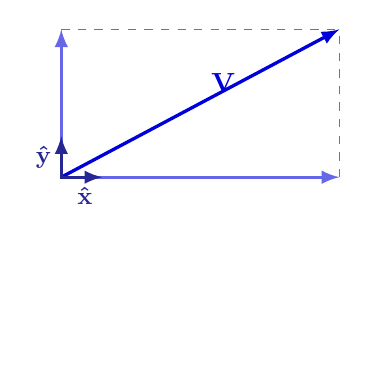
\begin{tikzpicture}
  \def\ul{0.52}
  \def\R{4}
  \def\ang{28}
  \coordinate (O) at (0,0);
  \coordinate (R) at (\ang:\R);
  \coordinate (X) at ({\R*cos(\ang)},0);
  \coordinate (Y) at (0,{\R*sin(\ang)});
  \draw[projcol,dashed] (X) -- (R);
  \draw[projcol,dashed] (Y) -- (R);
  \draw[vector] (O) -- (R) node[midway,left=5,above right=0] {$\vb{V}$};
  \draw[vector,<->,projcol]
    (X) node[scale=0.9,left=4,below=-1] {} -- (O) --
    (Y) node[scale=0.9,below=4,left] {};
  \draw[vector,<->,unitcol]
    (\ul,0) node[scale=0.9,left=2,below left=0] {$\vu{x}$} -- (O) --
    (0,\ul) node[scale=0.9,below=2,below left=0] {$\vu{y}$};
\end{tikzpicture}
$$

$$
V=\langle V, X\rangle\:\vu{x}+\langle V,Y\rangle\:\vu{y}
$$
Now, consider the infinite dimensional orthogonal basis $\{1\}\cup\{\cos(kx),\sin(kx)\}_{k=1}^{\infty}$. On this basis, we can write any periodic function as,

$$\boxed{f(x)=\frac{\langle f(x),1 \rangle}{\langle 1,1 \rangle}\cdot 1+\sum_{k=1}^{\infty}\frac{\langle f(x),\cos(kx) \rangle}{\langle \cos(kx),\cos(kx) \rangle}\cdot \cos(kx)+\sum_{k=1}^\infty\frac{\langle f(x),\sin(kx) \rangle}{\langle \sin(kx),\sin(kx) \rangle}\cdot \sin(kx)}$$

\section{Derivation: Fourier Series complex form}
So, far we have,
\begin{align}
\label{sin_cos_formula}
    \begin{split}
        \cos\theta&=\frac{e^{ikx}+e^{-ikx}}{2}\\
        \sin\theta&=\frac{e^{ikx}-e^{-ikx}}{2i}\\
        &= \frac{ie^{ikx}-ie^{-ikx}}{-2}
    \end{split}
\end{align}
\begin{align*}
    f(x)&=\frac{A_0}{2}+\sum_{k=1}^\infty A_k\cos(kx)+\sum_{k=1}^\infty B_k\sin(kx)\\
    &\stackrel{\ref{sin_cos_formula}}{=} \frac{A_0}{2}+\sum_{k=1}^\infty A_k\frac{e^{ikx}+e^{-ikx}}{2}+\sum_{k=1}^\infty B_k\frac{-ie^{ikx}+ie^{-ikx}}{2}\\
    &=\frac{A_0}{2}+\sum_{k=1}^\infty\left(\frac{A_k-iB_k}{2}\right)e^{ikx}+\sum_{k=1}^\infty\left(\frac{A_k+iB_k}{2}\right)e^{-ikx}
\end{align*}
Now, we want to collect all summation into a single summation. But how? The main problem arises because the last term contains a negative exponent. We replace it with a dummy indices $-k\rightarrow k$, then we get,
\begin{align*}
    &= \underbrace{\frac{A_0}{2}}_{C_0}+\sum_{k=1}^\infty\underbrace{\left(\frac{A_k-iB_k}{2}\right)}_{C_k}e^{ikx}+\sum_{k=-1}^{-\infty}\underbrace{\left(\frac{A_{-k}+iB_{-k}}{2}\right)}_{C_{-k}}e^{ikx}\\
    &= \sum_{k=-\infty}^\infty C_k e^{ikx}
\end{align*}
So far, so good. But how do we compute the complex coefficient $C_k$? Here comes the inner product role. So, we have,
\begin{align}
\label{com_Fseries}
    f(x)=\sum_{k=-\infty}^\infty C_k e^{ikx}
\end{align}
We can multiply $e^{-imx}$ both side of \ref{com_Fseries} and integrate from $\pi$ to $\pi$. 
\begin{align*}
    \int_{-\pi}^\pi f(x) e^{-imx} \, dx &= \int_{-\pi}^\pi \sum_{k=-\infty}^\infty C_k e^{ikx} e^{-imx} \, dx \\
    &= \sum_{k=-\infty}^\infty C_k \underbrace{\int_{-\pi}^\pi e^{ikx} e^{-imx} \, dx}_{2\pi\delta^k_m} \\
    &= \sum_{k=-\infty}^\infty 2\pi C_k \delta^k_m \\
    &= 2\pi C_m
\end{align*}
From where we can grab our complex coefficient and rewrite it as,
$$
\boxed{C_k=\frac{1}{2\pi}\int_{-\pi}^\pi  f(x)e^{-ikx}dx}
$$
\qed
~\\
We can see how the integration give the $2\pi$ result. Suppose, we have $$\int_{-\pi}^\pi e^{ikx}dx$$. Let's find the integral for $k=0:$
\begin{align*}
    \int_{-\pi}^\pi e^{i0x}dx&=\int_{-\pi}^\pi dx\\
    &=2\pi
\end{align*}
And for $k\neq0:$
\begin{align*}
    \int_{-\pi}^\pi e^{ikx}dx&=\frac{1}{ik}\left(e^{ik\pi}-e^{-ik\pi}\right)\\
    &=\frac{1}{ik}\left(\cos(k\pi)+i\sin(k\pi)-\cos(-k\pi)-i\sin(-k\pi)\right)\\
    &= \frac{1}{ik}2i\underbrace{\sin{k\pi}}_{=0}\\
    &= 0 
\end{align*}


\section{Half range Fourier series}
A half-range Fourier series is a Fourier series defined on an interval $(0, L)$ rather than the interval $(-L, L)$.\\
Given a function $f(x)$, defined on the interval $(0, L)$, we obtain its half-range sine series by calculating the Fourier sine series of its odd extension
$$
f_o(x)= \begin{cases}f(x) & \text { if } 0<x<L \\ -f(-x) & \text { if } \quad-L<x<0\end{cases}
$$
The Fourier coefficients of $f_o(x)$ are $a_n=0$ and
$$
b_n=\frac{1}{L} \int_{-L}^L f_o(x) \sin \frac{n \pi x}{L} d x=\frac{2}{L} \int_0^L f(x) \sin \frac{n \pi x}{L} d x .
$$
This gives the half range sine series for $f(x)$ on $(0, L)$ as $f(x)=\sum_{n=1}^{\infty} b_n \sin \frac{n \pi x}{L}$.
Given a function $f(x)$, defined on the interval $(0, L)$, we obtain its half-range cosine series by calculating the Fourier cosine series of its even extension
$$
f_e(x)= \begin{cases}f(x) & \text { if } 0<x<L \\ f(-x) & \text { if } \quad-L<x<0\end{cases}
$$
The Fourier coefficients of $f_e(x)$ are $b_n=0$ and
$$
a_n=\frac{1}{L} \int_{-L}^L f_e(x) \cos \frac{n \pi x}{L} d x=\frac{2}{L} \int_0^L f(x) \cos \frac{n \pi x}{L} d x
$$
This gives the half range cosine series for $f(x)$ on $(0, L)$ as $f(x)=\frac{a_0}{2}+\sum_{n=1}^{\infty} a_n \cos \frac{n \pi x}{L}$.
For a given (physical) problem on an interval $(0, L)$ it is usually the boundary conditions that determine whether an odd extension and a half sine Fourier series or an even extension and a half cosine Fourier series is more appropriate.

\begin{center}
	\begin{forest}
		for tree={%
			align=center, %% ADDED
			edge path={\noexpand\path[\forestoption{edge}] (\forestOve{\forestove{@parent}}{name}.parent anchor) -- +(0,-12pt)-| (\forestove{name}.child anchor)\forestoption{edge label};}
		}
		[
		Fourier Series ($-L\leq x\leq L$)\\Use formula \ref{normal_FS},
		[Fourier Sine Series ($0\leq x\leq L$)\\Use formula \ref{FSS}]
		[Fourier Cosine Series ($0\leq x\leq L$)\\Use formula \ref{FCS}]
		]
	\end{forest}
\end{center}

\begin{align}
\label{normal_FS}
    \begin{split}
        f(x)&=\frac{A_0}{2}+\sum_{k=1}^\infty A_k\cos\left(\frac{kx\pi}{L}\right)+\sum_{k=1}^\infty B_k\sin\left(\frac{kx\pi}{L}\right)\\
        A_k &= \frac{1}{L} \int_{-L}^L f(x) \cos\left(\frac{kx\pi}{L}\right) dx\\
        B_k &= \frac{1}{L}\int_{-L}^L f(x) \sin\left(\frac{kx\pi}{L}\right) dx
    \end{split}
\end{align}

\begin{align}
\label{FSS}
    \begin{split}
        f(x)&=\sum_{k=1}^\infty B_k\sin\left(\frac{kx\pi}{L}\right)\\
        B_k &= \frac{1}{L} \int_{-L}^L f_{\text{odd}}(x) \sin\left(\frac{kx\pi}{L}\right) dx\\
        &= \boxed{\frac{2}{L} \int_{0}^L f(x) \sin\left(\frac{kx\pi}{L}\right) dx}
    \end{split}
\end{align}

\begin{align}
\label{FCS}
    \begin{split}
        f(x)&=\frac{A_0}{2}+\sum_{k=1}^\infty A_k\cos\left(\frac{kx\pi}{L}\right)\\
        A_k &=  \frac{1}{L} \int_{-L}^L f_{\text{even}} \cos\left(\frac{kx\pi}{L}\right) dx\\
        &= \boxed{\frac{2}{L} \int_{0}^L f(x) \cos\left(\frac{kx\pi}{L}\right) dx}
    \end{split}
\end{align}

\section{Pythagoras' formula in Fourier world!}

\begin{problem}
~\\
\begin{tcolorbox}[colback=red!5!white,colframe=red!75!black]
Determine the period of the function $y=7\sin^{2024}5x+21$.
\end{tcolorbox}
~\\
\end{problem}

\begin{problem}
~\\
\begin{tcolorbox}[colback=red!5!white,colframe=red!75!black]
Draw sketches of the following graphs:
\begin{itemize}
    \item $f(x)=3|\sin(x)|,0\leq x\leq2\pi$
    \item $\begin{cases}
        2\sin x&,0\leq x\leq\pi\\
        0&,\pi\leq x\leq2\pi
    \end{cases}$
    \item $\begin{cases}
        1&,0\leq x\leq\pi\\
        0&,\pi\leq x\leq2\pi
        \end{cases}$
\end{itemize}
\end{tcolorbox}
~\\
\end{problem}

\begin{problem}
~\\
\begin{tcolorbox}[colback=red!5!white,colframe=red!75!black]
Find the Fourier series expansion of the function $f(x)$,
$$
f(x)=\begin{cases}
    x&,0<x<\pi\\
    -x&,-\pi<x<0
\end{cases}
$$
\end{tcolorbox}
~\\
\end{problem}

\begin{problem}
~\\
\begin{tcolorbox}[colback=red!5!white,colframe=red!75!black]
Find the Fourier series expansion of the function $f(x)$,
$$
f(x)=\begin{cases}
    2&,0<x<\pi\\
    -2&,-\pi<x<0
\end{cases}
$$
\end{tcolorbox}
~\\
\end{problem}

\begin{problem}
~\\
\begin{tcolorbox}[colback=red!5!white,colframe=red!75!black]
Find the Fourier Sine series expansion of the function $f(x)$,
$$
f(x)=\cos x, 0\leq x\leq \pi
$$
\end{tcolorbox}
~\\
\end{problem}

\begin{problem}
~\\
\begin{tcolorbox}[colback=red!5!white,colframe=red!75!black]
Find the odd extension of $f(x)=\cos(x)$ on $[0,\pi]$, draw it and find the Fourier Sine Series of it. 
\end{tcolorbox}
~\\
\end{problem}


\begin{problem}
~\\
\begin{tcolorbox}[colback=red!5!white,colframe=red!75!black]
Find the even extension of $f(x)=1-x$ on $[0,\pi]$, draw it and find the Fourier Sine Series of it. 
\end{tcolorbox}
~\\
\end{problem}
\section{From Fourier series to Transform}
\begin{align}
\label{complx_ft}
        f(x)&=\sum_{k=-\infty}^\infty C_k e^{\frac{ikx\pi}{L}}
\end{align}

Where, $$C_k = \frac{1}{2L}\int_{-L}^L f(x)e^{\frac{-ik\pi x}{L}}dx.$$
Take 
\begin{align}
\label{freq_CFT}
    w=k\frac{\pi}{L}=k\Delta w.
\end{align}
Now, we want a find the Fourier series of a function which is not periodic, $L\rightarrow\infty$ which implies our $\Delta w\rightarrow 0$. Then our \ref{complx_ft} become, 

\begin{align*}
    f(x) &= \lim_{\Delta w\rightarrow 0 }\left( \sum_{k=-\infty}^\infty {\color{red}{C_k}} e^{iwx} \right)\\
    &= \lim_{\Delta w\rightarrow 0 }\left( \sum_{k=-\infty}^\infty \left[{\color{red}{\frac{\Delta w}{2\pi} \int_{-\frac{\pi}{\Delta w}}^{\frac{\pi}{\Delta w}} f(\xi)e^{i(k\Delta w)\xi} d\xi}} \right] e^{iwx} \right)\\
    &= {\color{blue}{\lim_{\Delta w\rightarrow 0 }\sum_{k=-\infty}^\infty}}\left(\left[{\color{red}{\frac{1}{2\pi} \int_{-\frac{\pi}{\Delta w}}^{\frac{\pi}{\Delta w}} f(\xi)e^{iw\xi} d\xi}} \right] e^{iwx} \right){\color{blue}{\Delta w}}\\
    &= {\color{red}{\frac{1}{2\pi}}}{\color{blue}{\int_{-\infty}^{\infty}}} \underbrace{\left[{\color{red}{\int_{-\infty}^\infty f(\xi) e^{-iw\xi}d\xi}}\right]}_{\vu{f}(w)} {\color{blue}{e^{iwx} dw}}
\end{align*}
From this, we can say that the Fourier transform of a given function $f(x)$ is nothing but the following integral,
$$
\boxed{\mathcal F\{f(x)\}=\int_{-\infty}^\infty f(x) e^{-iwx}dx}
$$
And we denoted it by $\vu{f}(\omega)$. Similarly, for inverse Fourier Transform of given $f(x)$ is the following integral,
$$
\boxed{\mathcal F^{-1}\{f(x)\}=\frac{1}{2\pi}\int_{-\infty}^\infty f(x) e^{iwx}dw}
$$
Voila! We just derive the formula.
\qed\\
That means when we try to find the Fourier series of an aperiodic function we end up with the Fourier transform, Voila!\\
By the way, some authors distribute the $2\pi$ differently. Which creates slightly different looks for these formulas like:
$$
f(x)=\cdots={\color{red}{\frac{1}{\sqrt{2\pi}}}}{\color{blue}{\int_{-\infty}^{\infty}}} \underbrace{\left[{\color{red}{\frac{1}{\sqrt{2\pi}}\int_{-\infty}^\infty f(x) e^{-iwx}dx}}\right]}_{\vu{f}(w)} {\color{blue}{e^{iwx} dw}}
$$
Which implies,
$$
\boxed{\mathcal F\{f(x)\}=\frac{1}{\sqrt{2\pi}}\int_{-\infty}^\infty f(x) e^{-iwx}dx}
$$
$$
\boxed{\mathcal F^{-1}\{f(x)\}=\frac{1}{\sqrt{2\pi}}\int_{-\infty}^\infty f(x) e^{iw\xi}dw}
$$
Like our Fourier Series discussion, we can also see how odd or even functions can change the formula a bit.\\
If our $f(x)$ is an even function then, 
\begin{align}
\label{dum_cop}
\begin{split}
\mathcal{F}\{f(x)\}&=\int_{-\infty}^{\infty} f(x)e^{-i\omega x} \ dx \\
&=\int_{-\infty}^{\infty} f(x)\left(\cos(\omega x)-i\sin(\omega x)\right) \ dx \\
&=\int_{-\infty}^{\infty}\underbrace{f(x)\cos(\omega x)}_{\text{even function}} \ dx-\frac{i}{\sqrt{2\pi}}\int_{-\infty}^{\infty}\underbrace{f(x)\sin(\omega x)}_{\text{odd function}} dx \\
&={\color{blue}{2}}\underbrace{\int_0^{\infty} f(x) \cos(\omega x)  \ dx}_{\mathcal{F}_c\{f(\omega\}}
\end{split}
\end{align}
Doing the same computation for inverse Fourier transform we get,
\begin{align*}
    \mathcal F^{-1}(f(x))&=\frac{1}{2\pi}\int_{-\infty}^\infty f(x)e^{i\omega x}dx\\
    &=\vdots\\
    &= \frac{1}{2\pi}\int_{-\infty}^\infty f(x)\cos(\omega x)d\omega\\
    &= {\color{red}{2}}\frac{1}{2\pi}\int_{-\infty}^\infty f(x)\cos(\omega x)d\omega\\
    &\stackrel{\ref{dum_cop}}{=}\frac{{\color{blue}{2}}\cdot{\color{red}{2}}}{2\pi}\int_{-\infty}^\infty f(x)\cos(\omega x)d\omega\\
    &= \underbrace{\frac{2}{\pi}\int_{-\infty}^\infty f(x)\cos(\omega x)d\omega}_{\mathcal{F}^{-1}_c\{f(x)\}}
\end{align*}
Here, again we collect all coefficients in the inverse Fourier transform part. However, some authors distribute them equally. Okay, you can do the same computation for an odd function and get $\mathcal{F}_s\{f(x)\}$ and $\mathcal{F}^{-1}_s\{f(x)\}$.\\ 
For the sake of simplicity please use the following formula-tree to avoid confusion. 
\begin{center}
	\begin{forest}
		for tree={%
			align=center, %% ADDED
			edge path={\noexpand\path[\forestoption{edge}] (\forestOve{\forestove{@parent}}{name}.parent anchor) -- +(0,-12pt)-| (\forestove{name}.child anchor)\forestoption{edge label};}
		}
		[
		Fourier Transform\\Use formula \ref{normal_FT},
		[Fourier Sine Transform\\Use formula \ref{FST}]
		[Fourier Cosine Transform\\Use formula \ref{FCT}]
		]
	\end{forest}
\end{center}

\begin{align}
\label{normal_FT}
    \begin{split}
        \mathcal F\{f(x)\}&=\int_{-\infty}^\infty f(x) e^{-i\omega x}dx=\vu{f}(\omega)\\
        \mathcal F^{-1}\{\vu f(\omega)\}&=\frac{1}{2\pi}\int_{-\infty}^\infty \vu{f}(\omega) e^{i\omega x}d\omega
    \end{split}
\end{align}

\begin{align}
\label{FST}
    \begin{split}
        \mathcal F_s\{f(x)\}&=\int_{0}^\infty f(x) \sin(\omega x)dx=\vu{f}_s(\omega)\\
        \mathcal F^{-1}_s\{\vu f_s(\omega)\}&=\frac{2}{\pi}\int_{0}^\infty \vu{f}_s(\omega)\sin(\omega x)d\omega
    \end{split}
\end{align}

\begin{align}
\label{FCT}
    \begin{split}
        \mathcal F_c\{f(x)\}&=\int_{0}^\infty f(x) \cos(\omega x)dx=\vu{f}_c(\omega)\\
        \mathcal F^{-1}_c\{\vu f_c(\omega)\}&=\frac{2}{\pi}\int_{0}^\infty \vu{f}_c(\omega)\cos(\omega x)d\omega
    \end{split}
\end{align}
So, why is there $\frac{2}{\pi}$ in the inverse formula? Because we split our integral (because of eveness) twice: first in the $\mathcal F_c$ and second in the $\mathcal F_c^{-1}$. Hence, total factor increased by four times. We just collect this scaling and put inside the inverse formula,
\begin{align*}
    2\left(\frac{1}{2\pi}\int_{-\infty}^{\infty}\cdots\right)\rightarrow2\left(\frac{2}{2\pi}\int_{0}^{\infty}\cdots\right)\rightarrow\left(\frac{2}{\pi}\int_{-\infty}^{\infty}\cdots\right) 
\end{align*}
To make your life easy remember the following formulas:
$$\boxed{\int e^{ax}\cos bx\;dx = \frac{e^{ax}}{a^2+b^2}(a\cos bx+b\sin bx)}$$
$$\boxed{\int e^{ax}\sin bx\;dx = \frac{e^{ax}}{a^2+b^2}(a\sin bx - b\cos bx)}$$
You can find the full derivation \href{https://math.stackexchange.com/a/1502079}{here}.\\
\clearpage
\section{Unknotting the Interval mess up}
Okay, how do we calculate the upper and lower limits of the integration used in the Fourier series or transform part?  We always integrate the function in the given domain because our function is defined in that space. Actually, we do the periodic extension and then find the Fourier series. Like for the function, $f(x)=\begin{cases}
    1, & 0 < x < \pi\\
    -1, &-\pi < x < 0
\end{cases}$

\begin{figure}[H]
    \centering
    \includegraphics[width=\linewidth]{F_extend.png}
    \caption{Periodic extension}
    \label{fig:periodic_extend}
\end{figure}

So, basically, if you ask for the Fourier series, just make sure to find the interval of the function using the $2L$ formula, $$2L=\textbf{Given domain of the function}$$
And then use it in the general formula of the Fourier series:

\begin{align*}
    f(x)&=\frac{a_0}{2}+\sum_{k=1}^\infty a_k\cos{\left(k\frac{\pi x}{L}\right)}+\sum_{k=1}^\infty b_k\sin{\left(k\frac{\pi x}{L}\right)}\\
    a_0 &= \frac{1}{L}\int_{-L}^L f(x) dx\\
    a_k &= \frac{1}{L}\int_{-L}^L f(x) \cos{\left(k\frac{\pi x}{L}\right)} dx\\
    b_k&=  \frac{1}{L}\int_{-L}^L f(x) \sin{\left(k\frac{\pi x}{L}\right)} dx
\end{align*}
For example,
\begin{example}
Find the Fourier series expansion of the function $f(x)$ over the interval,
\begin{itemize}
    \item $(-\pi,\pi)$
    \item $(0,2\pi)$
    \item $(-4,4)$
    \item $(0,8)$
\end{itemize}
\textbf{Solution:} The value of $L$ is half of the length of the given interval.
\begin{itemize}
    \item For $(-\pi,\pi)$, $2L=\pi-(-\pi)=2\pi\Rightarrow L=\pi$
    $$\frac{1}{\pi}\int_{-\pi}^\pi ... dx$$ 
    \item For $(0,2\pi)$, $2L=2\pi-0=2\pi\Rightarrow L=\pi$
    $$ \frac{1}{\pi}\int_{0}^{2\pi} ... dx$$
    \item For $(-4,4)$, $2L=4-(-4)=8\Rightarrow L=4$
    $$ \frac{1}{4}\int_{-4}^{4} ... dx$$
    \item For $(0,8)$, $2L=8-0=8\Rightarrow L=4$
    $$ \frac{1}{4}\int_{0}^{8} ... dx$$
\end{itemize} 
\end{example} 
But if you asked for the Fourier Sine or Cosine series, then your formula gets changed as,
$$L=\textbf{Given domain of the function}$$
Because, this time we make it Odd or Even extension and then find the normal periodic extension and hence find the Fourier series.

\begin{figure}[H]
    \centering
    \includegraphics[width=1\linewidth]{images/Extension_odd_even.png}
    \caption{Odd or Even extension}
    \label{fig:odd-even_extend}
\end{figure}

And then use it in the general formula of the Fourier Sine series:

\begin{align*}
    f_s(x)&=\sum_{k=1}^\infty b_k\sin{\left(k\frac{\pi x}{L}\right)}\\\\
    b_k&=\frac{1}{L}\int_{-L}^L \underbrace{f(x) \sin{\left(k\frac{\pi x}{L}\right)}}_{odd\cdot odd=even} dx\\
    &\stackrel{eveness}{=}  \frac{2}{L}\int_{0}^L f(x) \sin{\left(k\frac{\pi x}{L}\right)} dx
\end{align*}
Here, $a_0,a_k=0$ because $f(x)$ is an odd (extended) function and $\cos{\left(k\frac{\pi x}{L}\right)}$ is an even function, hence their product is an odd function. And we know that, integrating an odd function in a complete period gives zero as the signed areas cancel each other.  
Fourier Cosine series:

\begin{align*}
    f_c(x)&=\frac{a_0}{2}+\sum_{k=1}^\infty a_k\cos{\left(k\frac{\pi x}{L}\right)}\\
    a_0 &= \frac{2}{L}\int_{-L}^L f(x) dx\\
    &= \frac{1}{L}\int_{-L}^L \underbrace{f(x) \cos{\left(k\frac{\pi x}{L}\right)}}_{even\cdot even=even} dx\\
    &\stackrel{eveness}{=} \frac{2}{L}\int_{0}^L f(x) \cos{\left(k\frac{\pi x}{L}\right)} dx
\end{align*}
Similarly, $b_k=0$ is also zero because,
$$
\tilde f(x)\sin{\left(k\frac{\pi x}{L}\right)}=\text{even (extended) function}\cdot\text{odd function}=\text{odd function}
$$
\begin{example}
Find the Fourier Sine series expansion of the function $f(x)$ over the interval,
\begin{itemize}
    \item $(0,\pi)$
    \item $(0,2\pi)$
    \item $(0,4)$
    \item $(0,8)$
    
\end{itemize}
\textbf{Solution:} The value of $L$ is the same as the length of the given interval.
\begin{itemize}
    \item For $(0,\pi)$, $L=\pi$
    $$ \frac{2}{\pi}\int_{0}^{\pi} ... dx$$
    \item For $(0,2\pi)$, $L=2\pi$
    $$ \frac{2}{2\pi}\int_{0}^{2\pi} ... dx$$
    \item For $(0,4)$, $L=4$
    $$ \frac{2}{4}\int_{0}^{4} ... dx$$
    \item For $(0,8)$, $L=8$
    $$ \frac{2}{8}\int_{0}^{8} ... dx$$
\end{itemize}
\end{example}
\clearpage 
\begin{problem} 
~\\
\begin{tcolorbox}[colback=red!5!white,colframe=red!75!black]
Given that, $$f(x)=\begin{cases}
    1,& |x|<a\\
    0,&|x|>a
\end{cases}$$
Use Fourier transform to find, $$\int_{-\infty}^\infty \frac{\sin(\omega a)\cos(\omega x)}{\omega}d\omega$$
Use your result to find, $$\int_{-\infty}^\infty\frac{\sin(x)}{x}dx=\frac{\pi}{2}$$
\end{tcolorbox}
~\\
\end{problem}

\begin{problem} 
~\\ 
\begin{tcolorbox}[colback=red!5!white,colframe=red!75!black]
Given that, $$f(x)=\begin{cases}
    1-x,& |x|<1\\
    0,&|x|>1
\end{cases}$$
Use Fourier transform to find, $$\int_{0}^\infty\left(\frac{x\cos(x)-\sin(x)}{x^3}\right)\cos{\frac{x}{2}}dx$$
\end{tcolorbox}
~\\
\end{problem}

\begin{problem} 
~\\ 
\begin{tcolorbox}[colback=red!5!white,colframe=red!75!black]
Given that, $$f(x)=\begin{cases}
    1,& 0<x<1\\
    0,&x\geq1
\end{cases}$$
Find Fourier Sine and Cosine transform of $f(x)$.
\end{tcolorbox}
~\\
\end{problem}

\clearpage


\printbibliography
\end{document}




